\documentclass{ieeeaccess}
\usepackage[usenames,dvipsnames]{xcolor}

%\definecolor{cincinnati-red}{RGB}{190,0,0}
\usepackage{cite}
\usepackage{amsmath,amssymb,amsfonts}
\usepackage{algorithmic}
\usepackage{graphicx}
\usepackage{textcomp}
\usepackage{float}
% \usepackage[utf8]{vietnam} 
\usepackage{xurl}
\usepackage{url}
\usepackage{subcaption}
\usepackage{comment}
\usepackage{dsfont}

\newcommand{\datta}[1]{\textcolor{blue}{#1}}
\newcommand{\baobq}[1]{\textcolor{orange}{#1}}
\newcommand{\anhvd}[1]{\textcolor{purple}{#1}}
\newcommand{\congtt}[1]{\textcolor{red}{#1}}
\def\BibTeX{{\rm B\kern-.05em{\sc i\kern-.025em b}\kern-.08em
    T\kern-.1667em\lower.7ex\hbox{E}\kern-.125emX}}
\begin{document}
\history{Date of publication xxxx 00, 0000, date of current version xxxx 00, 0000.}
\doi{10.1109/ACCESS.2017.DOI}

\title{Integrative Few-Shot Classification and Segmentation for Landslide Detection}
\author{\uppercase{Dat Tran-Anh}\authorrefmark{1}\textsuperscript{\textsection},
\uppercase{Bao Bui-Quoc\authorrefmark{2}\textsuperscript{\textsection}, Anh Vu-Duc\authorrefmark{1}, Trung-Anh Do\authorrefmark{1}, Hung Nguyen-Viet\authorrefmark{1}, Hoai-Nam Vu\authorrefmark{1} and Cong Tran\authorrefmark{1}}}
\address[1]{Posts and Telecommunications Institute of Technology, Hanoi, Vietnam}
\address[2]{Hanoi University of Science and Technology, Hanoi, Vietnam}

\tfootnote{This work was supported by the Qualcomm and PTIT Research Collaboration grant funded by Qualcomm (SOW Number POS-459341).
}

\markboth
{Author \headeretal: Preparation of Papers for IEEE TRANSACTIONS and JOURNALS}
{Author \headeretal: Preparation of Papers for IEEE TRANSACTIONS and JOURNALS}


\corresp{Corresponding author: Cong Tran (e-mail: congtt@ptit.edu.vn).}

% \footnotetext{Equal contribution}

\begin{abstract}
There has been an ongoing demand for monitoring landslides due to the heavy economic losses and casualties caused by such natural disasters. In this paper, we introduce a swift landslide detection system that can detect and segment landslides occurring on roads. To tackle the challenges of data collection, we propose an {\em automatic annotation procedure} to create a new landslide dataset consisting of 2963 images, termed the LandslidePTIT dataset. Additionally, we construct a novel deep-learning architecture that can perform both classification and segmentation tasks well from a few annotated images of landslides. Specifically, the model consists of four main modules that are delicately designed to solve the {\em few-shot segmentation} problem using landslide images, namely hypercorrection construction, attentive squeeze block, a cross-feature layer, and broadcast and squeeze layer. Experimental results exhibit the superiority of the proposed method in comparison with competitive baselines, in terms of both quantitative and qualitative manners.
\end{abstract}

\begin{keywords}
Data generation, few-shot learning, few-shot segmentation, image segmentation, landslide detection. 
\end{keywords}

\titlepgskip=-15pt

\maketitle
\begingroup\renewcommand\thefootnote{\textsection}
\footnotetext{Equal contribution}
\endgroup

\section{Introduction}
\label{sec:introduction}

\PARstart{L}{andslides}, typically a consequence of climate change \cite{Bourenane2021} and urban expansion \cite{Picarelli2021}, are one of the most common natural disasters today and cause severe troubles to human life and infrastructures all over the world. For example, a severe landslide occurred in mid-2020 in Vietnam, causing dozens of deaths.\footnote{Source: https://blogtuan.info/2022/05/20/serious-landslide-on-the-route-da-lat-mui-ne/} Landslides cause roads to be blocked, which causes hurdles not only in the traffic flow but also generate various traffic problems in the form of congestion \cite{Hung2015}.   Therefore, there is a need to detect and warn of landslides as quickly as possible to identify proper counter-measures so that possible unfortunate consequences can be avoided. 

Previous studies deal with two related problems of landslides, termed landslide detection and landslide prediction, in which the methods built upon machine learning and deep learning are quite common \cite{Ma2021, Tehrani2022}. However, practical applications of such methods are often limited due to the fact that deep learning models often require enormous labeled data to work well while landslides may only occur several times a year, thus it may take years to collect a sufficient amount of data. Besides, as landslides tend to occur in mountainous areas, collecting landslide images is difficult due to the danger as well as the lack of equipment in such underdeveloped areas. Several prior works tackle this problem by relying on images captured by satellites \cite{Prakash2021, Ghorbanzadeh2021}, which are however unable to respond promptly to a real-life landslide event unless we own the satellites.



\begin{figure*}[t]
  \centering
  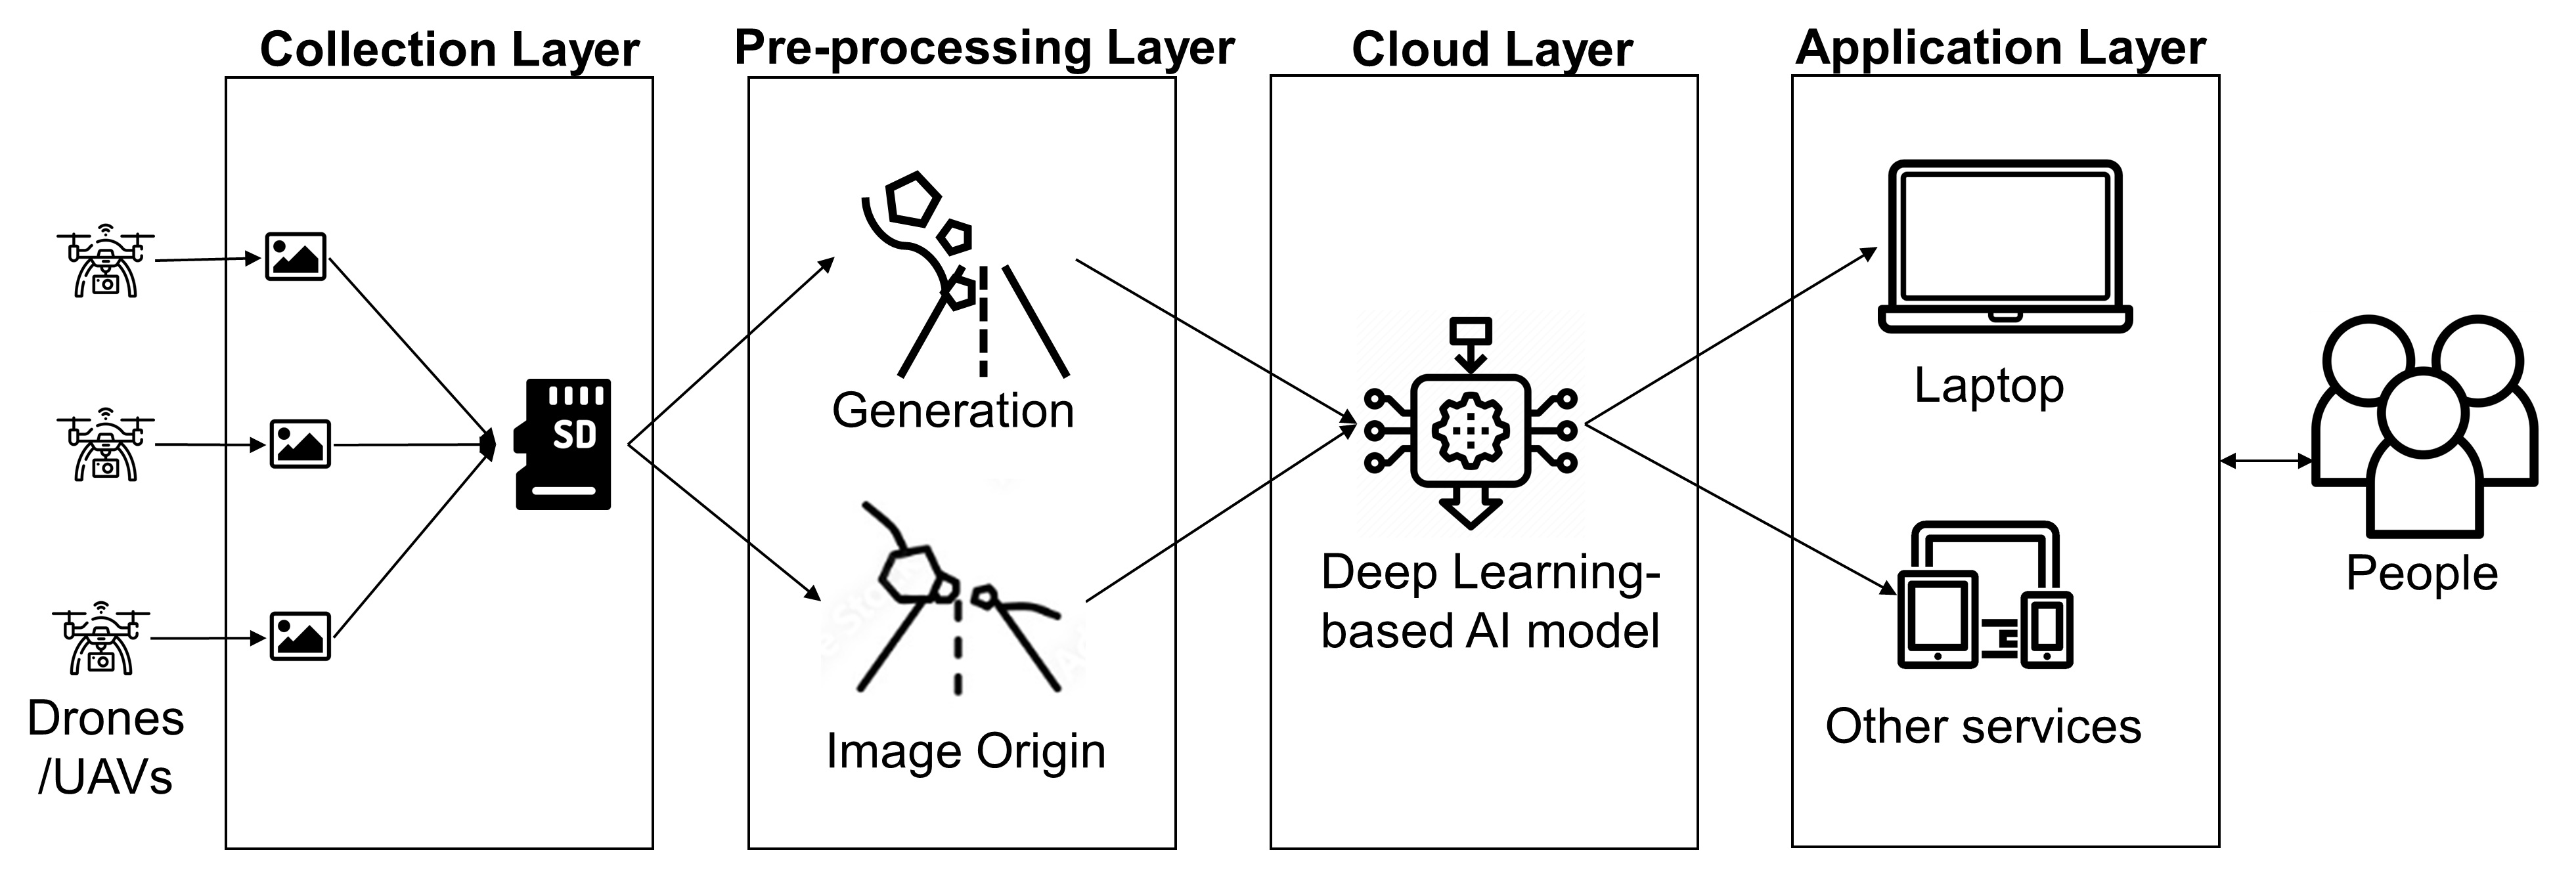
\includegraphics[width=\textwidth]{Fig/overview-system-landslide.png}
  % \caption{e-Landslide monitor architecture with four layers}
  \caption{Landslide detection systems with four layers}
  \label{fig-system}
\end{figure*}


In our work, we introduce a landslide monitoring system that can detect quickly whether there is any landslide occurring on roads. Fig. \ref{fig-system} illustrates our newly designed system consisting of four layers, namely collection, pre-processing, cloud, and application layers. Specifically, the system deploys specialized drones to collect images on roads in different areas, inspired by several recent novel methods that enables an energy-efficient routing schedule for capturing road images by drones  \cite{lui2022modelling,lui2021modelling}. As one of our main contributions, we propose a data generation procedure, where the generated images are pre-processed and annotated automatically. The generated images are fuel to train a deep learning-based artificial intelligence (AI) model in the cloud layer that can rapidly detect landslides causing damages on roads. After heavy rain stops, the operators deploy the drones to scan the surveillance areas and transfer the images to the AI model. The locations of landslides are then detected and extracted to create a map in the application layer for immediate response of local governors. 
It is worth noting that even with the pre-processing layer that generates images for training, it is still challenging to train the model well due to two reasons. First, the landslide can occur in any part of the roads, making it impossible for the data generation module to exhaustively generate landslides in every possible position for training. Second, the augmented landslides from generated images may not be generalized in real practice due to different types of landslides. Thus, as another important contribution, we propose a novel detection and segmentation method based on few-shot learning. In particular, the 
proposed method termed Cross Feature and Attentive Squeeze Network (CF-ASNet), combines the recently state-of-the-art ASNet model with the cross-validation method. By virtue of the transferability between few-shot learning classification and few-shot learning segmentation tasks, the classification and segmentation accuracy are greatly boosted.

Our contributions are four folds and are summarized as follows:
\begin{itemize}
    \item We introduce a new landslide detection system that aims to swiftly identify and measure the damage caused by landslides;
    \item We propose a novel data generation procedure, where labels of landslides are automatically assigned for training;
    \item We design a new model that can generalize to new types of landslides based on few-shot segmentation techniques;
    \item We empirically validate the effectiveness of the proposed data generation procedure as well as the newly designed model.
\end{itemize}


The organization of this paper is as follows. Section II presents relevant previous studies. In Section III, we describe the process of collecting landslide data to create our new dataset for training and testing landslides in two tasks, including detection and classification. In Section IV, we introduce a deep learning model for landslide detection based on a few-shot segmentation approach. Finally, we evaluate the proposed methods in section V.








\section{Related Work}
\label{relatedwork}
Our study is related to three broad categories, namely landslide detection, landslide segmentation and few-shot learning.
\subsection{Landslide Detection} 

{\bf Machine learning-based approaches}. Machine learning techniques used in landslide detection can follow both supervised and unsupervised settings. In supervised learning, typical methods employed support vector machine (SVM) \cite{Haojie2021,Milos2009}, k-nearest neighbors (KNN) \cite{Milos2009}, Logistic Regression (LR),Random Forest (RF) \cite{Milos2009, ChanW2014} and several other conventional classification techniques like Decision Tree\cite{Chandra2012}, Naive Bayes\cite{Ilia2016}, EML\cite{Lian2014}. These studies aimed at finding the relationship between known input and unknown output to classify each image with two labels, so-called ``landslide" or ``non-landslide".  In unsupervised methods, landslide samples are grouped based on their similarity. In \cite{Badal2020}, the authors proposed an unsupervised method by utilizing six unsupervised well-known methods, including K-means, K-medoids, hierarchical cluster (HC) analysis, expectation–maximization using Gaussian mixture models (EM/GMM), affinity propagation, and mini-batch K-means, to find cluster pattern of landslides, which then acts as training data for the landslide detection problem.

{\bf Deep learning-based approaches}.
The convolutional neural network (CNN) is the most common technique for these approaches. A recent study on landslide identification \cite{Haojie2021} showed that CNN outperforms most machine learning-based approaches such as RF, LR, and SVM. Bui et al. \cite{TrongAn2020} proposed a system combining CNN for classification tasks and a transformation algorithm Hue - Bi-dimensional empirical mode decomposition (H-BEMD) to locate the landslide region and size. Interestingly, this study ferreted out that the landslide size depends on time. Another approach proposed in \cite{HongYu2017} combined CNN and a region-growing algorithm for two main tasks: detecting and classifying the landslide, which reached 97\% in terms of F1 score. On other hand, time series data was also utilized to detect the structure changes \cite{Anzi2016}, where non-contribute areas including vegetation, water, and buildings were removed from the pre-landslide and post-landslide images, followed up by a CNN model to detect the changes in image patches.

\subsection{Landslide Segmentation} 
For landslide problems, semantic segmentation is a prevalent task. 
Several studies employed U-net  \cite{Unet2015}, which is the state-of-art deep learning model for semantic segmentation tasks, as the main method for landslide detection and segmentation. Landslide detection in the Himalayas from satellite images \cite{Sansar2022} compared the performance of U-net and common machine learning-based approaches on two popular datasets, including five optical bands from the RapidEye satellite images and ALOS-PALSAR derived topographical data. To evaluate the efficiency of the generalization model for various datasets, a survey of rainfall-induced landslides in Brazil \cite{Lucas2022} was performed on three datasets including RapidEye satellite images, Normalized Vegetation Index (NDVI), and a digital elevation model (DEM) figured out that the large patch size has better perform in detect landslides in areas similar to the training area and the small patch has more efficiency in landslide detection in areas with different environmental aspects. Li et al. \cite{HuajinLi2022} designed a two-phase framework: F-RCNN for detection and U-net for segmentation of landslide from satellite's images, where skip connection is deployed to replace inception block at the second phase of U-net architecture. Moreover, the authors in \cite{Zhunli2020} proposed another method that combines MobileNetV2 and PSPnet to accelerate the speed and reduce the number of parameters, which reduced the misclassification errors and separated the objects more precisely.

\subsection{Few-shot learning}
{\bf Few-Shot learning (FSL)} is a special case of meta-learning \cite{Joaquin2018}, which aims to train a model that can perform well with unseen data using a few samples under related tasks. The main idea of FSL is to determine a hypothesis space of hypotheses and estimates an optimal hypothesis. FSL included interesting variants such as one-short learning \cite{Mark2017, Brenden2011, Fei2006} that classifies each label with only one sample for each class and zero-shot learning \cite{Lampert2013, Larochelle2008, Rohrbach2011, Ding2017} that deals with unseen data using data description without any labeled samples. 

FSL has been widely adopted in classification, object detection, and recognition. For example, the authors in \cite{Dhillon2020, Chen2021} showed that FSL achieved better performance in hyperspectral images (HSI) classification, which typically requires hundreds or thousands of labeled samples. Following up, Liu et al. proposed deep few-shot learning for hyperspectral image classification \cite{Liu2019}, in which the crucial concept is to exploit the training dataset to provide a metric space that can generalize to the classes in the unseen dataset. The suggested approach achieved a higher classification accuracy than the traditional semi-supervised methods by evaluating four popular HSI data sets. 
Additionally, in object detection tasks, a class-imbalanced scenario was considered for road object detection using FSL \cite{Majee2021}, which demonstrated the application of few-shot learning approaches in real-world images under a driving context. Furthermore, in the recognition task, Das et al. proposed a two-stage approach based on few-shot learning for image recognition \cite{Das2019}.  In the first-training
stage, the authors captured the structure
of the data and obtained an embedding space while also predicting the variance of each class. In the second-training stage, the proposed method learned to map the mean-sample representation to class prototype representation in the embedding space.

{\bf Few-shot segmentation} \cite{Dong2018, Kaixin2019, Boudiaf2021} is a sub-field of few-shot learning, which utilized FSL in the segmentation tasks and was paid considerable attention in recent years. An early prototype learning for few-shot segmentation was proposed by Nanqing Dong \cite{Dong2018}. In that article, the authors introduced a framework based on prototype learning and metric learning that significantly outperformed the baselines on PASCAL VOC 2012 dataset.  Wang et al. proposed a novel prototype alignment network, termed PANet, that can effectively utilize the support set's data \cite{Kaixin2019}. Interestingly, PANet introduced the prototype alignment regularization between the support and query by providing a few-shot segmentation reversely from query to support. Most recently, a method of FSL without meta-learning was proposed in  \cite{Boudiaf2021}, which adopted only transductive inference technique for a given query image while taking advantage of the statistics of its unlabeled pixels by maximizing a new loss containing three complementary terms, including the 1) cross-entropy obtained from the labeled support pixels, 2) Shannon entropy of the posteriors on the unlabeled query-image pixels, and 3) a global KL-divergence regularizer. The method achieved competitive performances in the 1-shot learning setting  and noticeably improved performance in the 5- and 10-shot scenarios by 5\% and 6\%, respectively, in comparison with state-of-the-art episodic training approaches.

% Use either SI (MKS) or CGS as primary units. (SI units are strongly 
% encouraged.) English units may be used as secondary units (in parentheses). 
% This applies to papers in data storage. For example, write ``15 
% Gb/cm$^{2}$ (100 Gb/in$^{2})$.'' An exception is when 
% English units are used as identifiers in trade, such as ``3\textonehalf-in 
% disk drive.'' Avoid combining SI and CGS units, such as current in amperes 
% and magnetic field in oersteds. This often leads to confusion because 
% equations do not balance dimensionally. If you must use mixed units, clearly 
% state the units for each quantity in an equation.

% The SI unit for magnetic field strength $H$ is A/m. However, if you wish to use 
% units of T, either refer to magnetic flux density $B$ or magnetic field 
% strength symbolized as $\mu _{0}H$. Use the center dot to separate 
% compound units, e.g., ``A$\cdot $m$^{2}$.''
\section{Pre-processing Layer}
\label{sec:3}
In this section, we describe the data pre-processing step after obtaining images from UAVs/drones. A landslide is a dangerous natural phenomenon that occurs during heavy rain and floods and can cause a lot of damage to people and infrastructure. Furthermore, the landslide may block the whole road, causing traffic circulation obstruction. 
%In Viet Nam, the flood season on rivers from the North to the South Central region tends to appear later from north to south and mainly happens from June to December. When the flood season comes, landslides mostly occur in mountainous areas like in Lai Chau, Quang Nam, Hoa Binh, ... .
Due to difficulty in traffic conditions, terrain, and shortage of equipment such as UAVs and drones, it is challenging to collect data and thus the amount of collected data every year is very few. Since deep learning models typically require a huge amount of data to perform well, we need to generate more data to compensate for a limited number of collected images. 

To this end, we build a newly generated dataset via three following steps, namely data crawling, data generation, and data annotation. In the following, we present the three steps for generating landslide images and then building a landslide dataset including generated images and their annotations.

 
\begin{figure*}[!t]
\centering
  \begin{tabular}[b]{cc}
    \begin{tabular}[b]{c}
      \begin{subfigure}[b]{1.3\columnwidth}
        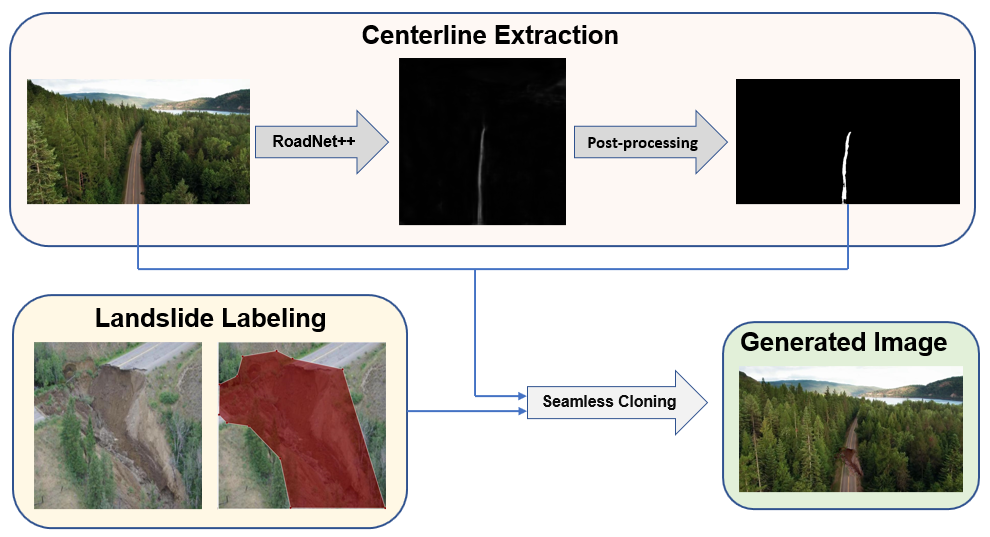
\includegraphics[width=\textwidth]{Fig/gen_landslide.png}
        \caption{Landslide image generation process.}%\congtt{add text on top of three boxes in the figure (centerline extraction, landslide labeling, generated image), replace cv2.seamlessClone with Seamless Cloning}}
        \label{fig:A}
      \end{subfigure}\\
      \begin{subfigure}[b]{1.3\columnwidth}
        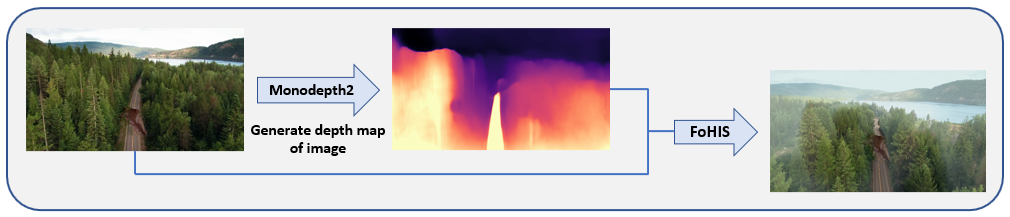
\includegraphics[width=\textwidth]{Fig/gen_fog.png}
        \caption{Fog generation process for data annotation.}
        \label{fig:B}
      \end{subfigure}
    \end{tabular}
    &
    \begin{subfigure}[b]{0.6\columnwidth}
      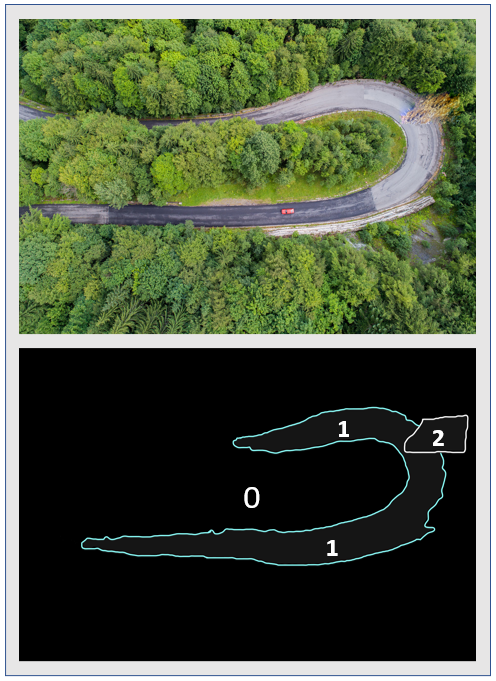
\includegraphics[width=\textwidth]{Fig/anno.png}
      \caption{Generated landslide image and its corresponding annotation.}
      \label{fig:C}
    \end{subfigure}
  \end{tabular}
  \caption{Examples of data generation and annotation steps in the pre-processing layer.}
  \label{fig:ABC}
\end{figure*}

\subsection{Data Crawling} 
We collect videos of road data recorded by UAV and drone, in several mountain and forest areas in Vietnam. Frames are extracted from videos and we obtain a dataset consisting of 767 road images. For landslide data, we collect 149 images from the internet by manually selecting landslide images that are taken from a high-ground position, which simulates the actual deployment situation when the UAVs/drones take pictures during surveillance. Then, we also annotate the images with many types of slides such as rock falls, mudslides, earth flow, and depression. The data statistics are shown in Tables \ref{tab:background-scene-type} and \ref{tab:landslide-type}.


\begin{table}[t]
\caption{Statistics of the number of road images by background scene.}
\centering
\begin{tabular}{|c|c|}
\hline
Background scene & Number of images \\ \hline
Forest only      & 290              \\ \hline
Forest mountain  & 116              \\ \hline
Rock mountain    & 361              \\ \hline
\end{tabular}
\label{tab:background-scene-type}
\end{table}

\begin{table}[t]
\caption{Statistics of the number of real-life landslide images by type.}
\centering
\begin{tabular}{|c|c|}
\hline
Types of landslide & Number of images \\ \hline
Rock fall          & 21               \\ \hline
Mud slide          & 29               \\ \hline
Earth flow         & 66               \\ \hline
Depression         & 33               \\ \hline
\end{tabular}
\label{tab:landslide-type}
\end{table}

\subsection{Data Generation and Augmentation}

In this section, we explain the procedure to generate images containing landslides that can be utilized to train machine learning/deep learning models. Each synthetically generated image contains a road augmented with a type of landslide listed in Table \ref{tab:classes}. 

To this end, we first need to determine the centerline of the road in road images and the landslide region in landslide images. For extracting the centerline, we adopt the pretrained RoadNet++ model \cite{liu2019roadnet} and then apply post-processing to the model output, resulting in a binary image with pixel value 1 corresponding to the centerline and 0 otherwise. For the landslide region, we crop out the region corresponding to the landslide from four types of landslide images using Labelme application.\footnote{Labelme image polygonal annotation tool: \url{https://github.com/wkentaro/labelme.git}} Finally, we randomly insert the landslide region on the centerline of the road in the image, using the Seamless Cloning algorithm \cite{matias2016Poisson-Image-Editing} 
method. The region is blended into the road image, making it more realistic. This above-mentioned procedure is illustrated in Fig. \ref{fig:A}. After conducting the data generation phase, from 767 and 149 collected road and landslide images, respectively, we obtain a generated dataset consisting of 2963 images, termed the LandslidePTIT dataset.

After a landslide occurs, light rain is typically observed in the surrounding area. Besides, the landslides tend to occur in mountainous areas, thus the images are often captured in foggy weather. To simulate these two weather conditions, we further augment fog and rain to generate images in the LandslidePTIT dataset, which divides the dataset into three parts normal, fog, and rain.\footnote{In this study, we generate fog using FoHIS (\url{https://github.com/noahzn/FoHIS}) and generate rain using monodepth2 (\url{https://github.com/nianticlabs/monodepth2}).}

\begin{comment}
\begin{figure*}
    \centering
    \begin{minipage}{.3\linewidth}
            \begin{subfigure}[t]{.9\linewidth}
                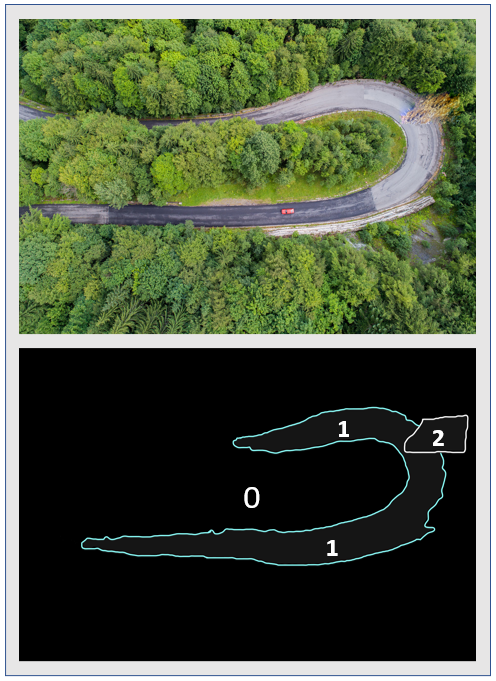
\includegraphics[width=\textwidth]{Fig/anno.png}
                \caption{Weergave gezochte routes}
                \label{fig:weather_activity}
            \end{subfigure}
        \end{minipage}
    \begin{minipage}{.6\linewidth}
        \begin{subfigure}[t]{1.05\linewidth}
            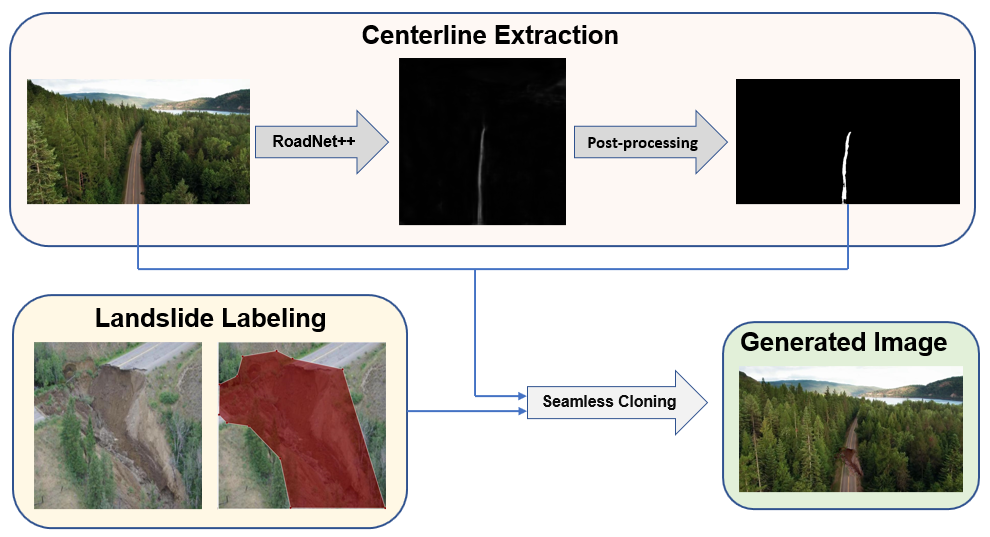
\includegraphics[width=\textwidth]{Fig/gen_landslide.png}
            \caption{Detail van een route}
            \label{fig:weather_filter1}
        \end{subfigure} \\
        \begin{subfigure}[b]{1.05\linewidth}
            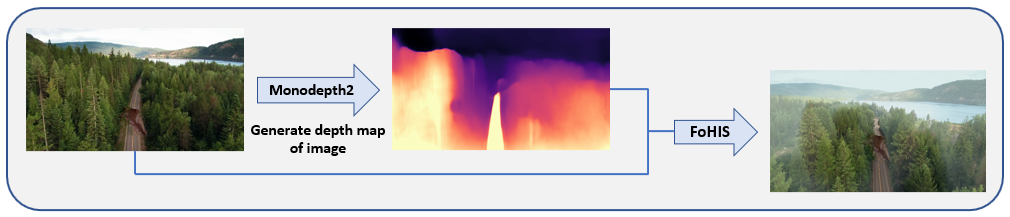
\includegraphics[width=\textwidth]{Fig/gen_fog.png}
            \caption{Detail van een route}
            \label{fig:weather_filter2}
        \end{subfigure} 
    \end{minipage}
    \caption{Many figures}
\end{figure*}
\end{comment}


\subsection{Data Annotation}
The images are labeled pixel-wise, i.e., each pixel of an image is annotated with a range of values from 0 to 255 that indicates the class number. For example, in Fig. \ref{fig:C}, id 0, 1, and 2 are background, road, and earth flow, respectively. Table \ref{tab:classes} presents the list of classes deployed in our study. The annotations are JSON files that store coordinates of the polygon forming the landslide area. 

\begin{table}[t]
\caption{Class information in the LandslidePTIT dataset.}
\centering
\begin{tabular}{|c|c|c|}
\hline
Class      & Id & Number of images \\ \hline
Background & 0  & 2963             \\ \hline
Road       & 1  & 2963             \\ \hline
Earth flow & 2  & 1190             \\ \hline
Depression & 3  & 596              \\ \hline
Mud slide  & 4  & 523              \\ \hline
Rock fall  & 5  & 379              \\ \hline
\end{tabular}
\label{tab:classes}
\end{table}

%\subsubsection{Rain Generation}
%\baobq{ }

\section{Cloud Layer}

In this layer, we design a model to tackle the landslide detection problem. Specifically, we need to answer the following questions. First, does a landslide appear in a given input image? Second, if a landslide occurs, then does it block the road and may obstruct traffic? Third, what is the class of landslides? Intuitively, if we know the current state of the landslide and the type of landslide, e.g., rockfall, mudslide, etc., then we can issue warnings and take appropriate action based on the situation. To answer these questions, we not only solve the classification task, which classifies an image as the type of having landslide or not but also need to locate the area on the road where the landslide takes place, which is equivalent to the segmentation problem. 

Besides, since collecting landslide data is challenging, it is difficult to acquire a large enough dataset to train on conventional deep learning models. Additionally, in reality, each region has different characteristics and there are many types of landslides other than those presented in our LandslidePTIT dataset. For example, in the northwest mountainous areas of Vietnam, the terrain is mainly high mountain forests. In this type of terrain, flash floods often occur and can be considered a new landslide type that we need to detect.

Therefore, we propose a few-shot segmentation framework to tackle the landslide detection problem, in which we also newly design a cross-feature attentive squeeze network architecture that is customized for the LandslidePTIT dataset.
\subsection{Problem Formulation}

Few-shot learning aims at performing tasks with only a few labeled data. In our study, we are given two image sets: 1) base set, denoted as $\mathcal{D}^T$ (with base classes), and 2) novel set, $\mathcal{D}^E$ (with novel classes). We note that the novel set also includes road and landslide images, however, the classes in the novel set are different from those in the base set. Specifically, in the training process, the LandslidePTIT dataset is divided into two parts as train set and test set, which are $\mathcal{D}^T$ and $\mathcal{D}^E$ respectively. We denote $\mathcal{C}^{T}$ and $\mathcal{C}^{E}$ as the class sets of $\mathcal{D}^T$ and $\mathcal{D}^E$, respectively. In the specific case of the LandslidePTIT dataset, we have $|\mathcal{C}^T| + |\mathcal{C}^E| = 6$.

%We split the dataset into parts with different background contexts; for example, images of roads in many kinds of regions (mountain, forest, highland, ...) or images with many types of roads like concrete, asphalt, earthen, ... . We can also classify the landslide into different types and assign them as new classes. We have two primary ways to classify the landslide: by the causes of the landslide (mudslide, rockfall, earth flow, ...) or by the damage of the landslide to the road (landslide - earth, rock or many kinds of things that fall down and block the road; depression - the geological layer below the road is affected, causing it to collapse and fracture). The models are expected to learn transferable knowledge on $I_{base}$ with sufficient annotated samples. The models are optimized during each training episode to make predictions on the query image under the condition of the support set. Once the training is complete, we will evaluate the performance on $I_{novel}$ across all the test episodes, without further optimization. In this work, we follow an integrative Few-Shot Learning framework [] that combined and generalized classification and segmentation task for our landslide detection problem.

To detect landslides under the few-shot setting, we follow the idea of episodic learning \cite{Li_2019_ICCV}, which is one of the most well-known approaches in the field. Specifically, multiple few-shot tasks are created in the training process, each takes several data samples randomly drawn from the train set $\mathcal{D}^T$ and divides the samples into two sets including a support set, denoted as $\mathcal{S}^T$, and a query set, denoted as $\mathcal{Q}^T$. 
The model performs the classification and segmentation of the data in the query set based on the data and labels information in the support set.
For each few-shot task in the training process, the support set $\mathcal{S}^T$ is a set that has information about the landslide and the corresponding labels while the query set $\mathcal{Q}^T$ includes images that are not labeled, i.e., we need to classify and segment roads and landslides from images in $\mathcal{Q}^T$. 

After training completely, we evaluate the model by using the test set $\mathcal{D}^E$ which is also the novel set. The support set $\mathcal{S}^E$ and the query set $\mathcal{Q}^E$ are taken from the test set as the way performed in the training process. We have to use a few-shot learning model to predict the labels of data samples in the query set. Also, during the inference process, the query set is the set of images obtained from the UAVs/drones in the field, which do not have label data and we need to predict the type of landslide and its landslide segmentation. The support set includes several images with a new type of landslide and their labels. 

In more detail, we create episodes containing two following sets of samples. 
\begin{itemize}
    \item $\mathcal{S}^{\ast}=\left\{\bigl(x^s_i, a^s_i\bigr) \bigm| x^s_i \in \mathbb{R}^{H \times W \times C}, a^s_i \in \mathbb{R}^{H \times W} \right\}_{i=1}^{N K}$, where $x^s_i$  and $a^s_i$ represent a support image with its label from $\mathcal{S}^{\ast}$, the superscript  $\ast$ represents $T$ and $E$ for train and test sets, respectively, $N$ is the number of classes in support set, and each class contains $K$ labeled instances, i.e., the so-called $N$-way $K$-shot problem. In particular, $x^s_i$ and $a^s_i$ represent a raw image and its corresponding label for a specific category, respectively. Each value in the annotation matrix $a^s_i$ is the class id of the corresponding pixel in image $x^s_i$. We also denote $H, W, C$ as height, width, and channels of the image $x^s_i$, respectively.
    \item $\mathcal{Q}^{\ast}=\left\{x^q_j \; | \; x^q_j \in \mathbb{R}^{H \times W \times C} \right\}_{j=1}^M$, where $x^q_j$ is a query landslide image and $M$ is a number of images in $\mathcal{Q}^{\ast}$ that needed to predict. The superscript  $\ast$ represents $T$ and $E$ for train and test sets, respectively, and $j$ indicates the $j$-th data samples in $\mathcal{Q}^{\ast}$. 
\end{itemize}

For classification task, we aim to identify the multi-hot class occurrence vector $\mathbf{y}_\mathbf{C} \in  \mathbb{R}^{N}$ via a function $f_\mathbf{C}$; and for segmentation task, we predict the segmentation mask $\mathbf{Y}_\mathbf{S} \in \mathbb{R}^{H \times W}$ corresponding to the classes via another function $f_\mathbf{S}$. The two objectives are expressed as follows:
\begin{equation}
\label{eq:1}
\begin{aligned}
   \mathbf{y}_\mathbf{C} &= f_\mathbf{C}(x^q_j, \mathcal{S}^* ; \theta_\mathbf{C}), \\
   \mathbf{Y}_\mathbf{S} &= f_\mathbf{S}(x^q_j, \mathcal{S}^* ; \theta_\mathbf{S}),
   \end{aligned}
\end{equation}
where $\theta_\mathbf{C}, \theta_\mathbf{S}$ are the learnable parameter of the classification model and the segmentation model, respectively. %\congtt{$\mathcal{S}$ is inconsistent with previous notations, Bao please correct the notation over all the manuscript}

In this study, instead of optimizing two functions $f_\mathbf{C}$ and $f_\mathbf{S}$ in (\ref{eq:1}) separately, we aim at jointly finding a function $f_\mathbf{CS}$ that combines and generalizes two tasks, including few-shot classification and segmentation (FS-CS). It can predict multi-label background-aware class occurrences and also segmentation maps. The integrative FS-CS model $f_\mathbf{CS}$ (with learnable parameter $\theta_\mathbf{CS}$) take as input query image $x^q_j$ and support set $\mathcal{S}^*$,
\begin{equation}
    \left\{\hat{\mathbf{y}}_{\mathbf{C}}, \hat{\mathbf{Y}}_{\mathbf{S}}\right\}=f_\mathbf{CS}(x^q_j, \mathcal{S}^* ; \theta_\mathbf{CS}),
    \label{eq2}
\end{equation}
where $\hat{\mathbf{y}}_{\mathbf{C}} \in \mathbb{R}^N$ is the multi-hot class occurrence vector and $\hat{\mathbf{Y}}_{\mathbf{S}} \in \mathbb{R}^{H \times W}$ is  the class-wise segmentation
mask.

We note that FS-CS is more general than few-shot classification (FS-C) and also exhibits two major advantages over both FS-C and few-shot segmentation (FS-S) as follows:
\begin{itemize}
  \item FS-CS can classify the query images, which are belonging to none or multiple target classes (i.e., the query is classified into a background class - none if none of the target classes were detected). Therefore, in a real-life use case, if a landslide does not occur, then the system still operates properly without any warnings.
  \item FS-CS relaxes the assumption such that the query class set can be a subset of the support class set while the conventional FS-S \cite{Kaixin2019}, \cite{PFENet}, \cite{HSNet} assumes the query class set exactly matches the support class set.
\end{itemize}


To solve (\ref{eq2}), we need to extract $N$ probability maps corresponding to each class in the support set, which is typically referred to as the class-wise foreground map set, $\mathcal{Y}$, comprised of $\mathbf{Y}^{(n)} \in \mathbb{R}^{H \times W}$ for $N$ classes. Where $\mathbf{Y}^{(n)}$ is the probability map of a class (each position on the map represents the probability of the position being on a foreground region of the corresponding class) and has the same size as the input image $H \times W$. We have:
\begin{equation}
\label{eq:probform}
\mathcal{Y}=f(x^q_j, \mathcal{S}^* ; \theta)=\left\{\mathbf{Y}^{(n)}\right\}_{n=1}^{N},
\end{equation}
where $f$ is the model before the post-processing step and $\theta$ is the learnable parameter of the model. $\mathcal{Y}$ is then post-processed to extract $\hat{\mathbf{y}}_{\mathbf{C}}$ and $\hat{\mathbf{Y}}_{\mathbf{S}}$ (see Section IV.C.1 for further details).

\subsection{Model Architecture}
\label{ModelArch}

%%%%%%%%%%%%%%%%%%%%%%%%%%%
\begin{comment}
To solve (\ref{eq:probform}), we propose a new model architecture, termed CF-ASNet, built upon the state-of-the-art ASNet model \cite{Kang2022}. The overall procedure of CF-ASNet is presented in Fig. \ref{fig-system}. As illustrated in the figure, we first extract feature maps of a query image (depicted in red) and a support image (depicted in green). Each pair of feature maps (with the same level) are then used to construct hypercorrelations, which is depicted as two 2D-squares. The model then learns to transform the correlation to a foreground map by gradually squeezing the support dimension on each query dimension. While transforming, two adjacent correlation in intermediate correlation level are cross featured. The detailed implementations are described in the following subsections.
\end{comment}
%%%%%%%%%%%%%%%%%%%%%%%%%%%

To solve (\ref{eq:probform}), we propose a new model architecture, termed CF-ASNet, built upon the state-of-the-art ASNet model \cite{Kang2022}. The overall procedure of CF-ASNet is presented in Fig. \ref{fig:arch}. As illustrated in the figure, we first extract feature maps of a query image (depicted in red) and a support image (depicted in green) from a backbone network, which is illustrated by a trapezoid shape.\footnote{In this paper, we adopt ResNet50 as the backbone network.} In this backbone network, three features of an image are extracted from the three last blocks, i.e., blocks 2, 3, and 4 in Fig. \ref{fig:arch}. Each feature maps pairs with the same level are then used to construct hypercorrelations - the first pyramidal correlation box in the figure. Secondly, the model then learns to transform the correlation through an attentive squeeze block whose details are presented in Fig. \ref{fig:asblock} by gradually squeezing the support dimension on each query dimension, yielding the high-level hypercorrelations that are later employed to produce the mask prediction map. Finally, in the producing process, two adjacent correlations are cross featured using a network termed the cross feature layer. Each high-level correlation tensor pair after processing results in a feature map, is upsampled and combined with the same query dimension size correlation using broadcast and squeeze layers, whose details are described in Sections \ref{CFlayer} and \ref{BSlayer}, respectively. The earliest feature map is fed to a convolutional decoder, which consists of bi-linear upsampling and interleaved 2D convolution that map the number of dimensional channels to 2 (including foreground and background) and the output spatial size to the input query image size. The detailed implementations are described in the following subsections.


    \begin{figure*}[t]
        % \caption{{Overview of the proposed Few-shot CF-AS Network}}
        \centering
        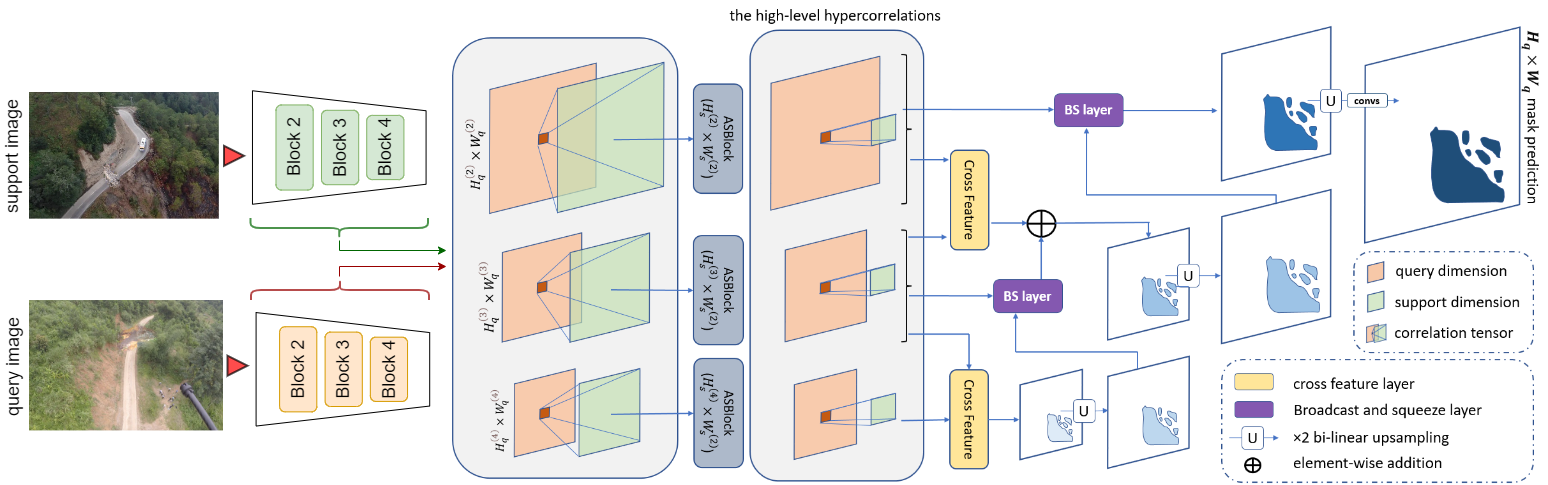
\includegraphics[width=\textwidth]{Fig/landslide-model.png}
        % \caption{Overview of the proposed Few-shot CF-AS Network}
        \caption{\textbf{Overview of the proposed Cross Feature and Attentive Squeeze Network (CF-ASNet)}}
        \label{fig:arch}
    \end{figure*}

\subsubsection{Hypercorrelation Construction}
Following \cite{HSNet}, we construct hypercorrelations between the query image and the support image. First, we extract the features of each image from a pre-trained backbone network (the pre-trained  is frozen during the training process). We denote $\mathbf{F}_{q}^{(b)} \in \mathbb{R}^{C^{(b)} \times H^{(b)}_{q} \times W^{(b)}_{q}} , \mathbf{F}_{s}^{(b)} \in \mathbb{R}^{C^{(b)} \times H^{(b)}_{s} \times W^{(b)}_{s}}$ are feature maps of the query image and the support image from block $b$ of the backbone model ($H^{(b)}_{*}, W^{(b)}_{*}$ are the feature map size and $C^{(b)}$ is the number of channels). In our work, we adopt ResNet50 and ResNet101 pre-trained as feature extractors, with the output channel sizes of four blocks set to \{3, 4, 6, 3\} and \{3, 4, 23, 3\}, respectively. The feature maps pairs of query and support image from block 2, block 3 and block 4 - $\{(\mathbf{F}_{q}^{(b)}, \mathbf{F}_{s}^{(b)})\}_{b=2}^4$ are then used  to compute cosine similarity as follow: 
\begin{equation}
\textbf{\mathfrak{C}}^{(b)}\left(\mathbf{p}_{q}, \mathbf{p}_{s}\right)=\operatorname{ReLU}\left(\frac{\mathbf{F}_{q}^{(b)}\left(\mathbf{p}_{q}\right) \cdot \mathbf{F}_{s}^{(b)}\left(\mathbf{p}_{s}\right)}{\left\|\mathbf{F}_{q}^{(b)}\left(\mathbf{p}_{q}\right)\right\|\left\|\mathbf{F}_{s}^{(b)}\left(\mathbf{p}_{s}\right)\right\|}\right),
\end{equation}
\begin{equation*}
\mathbf{p}_q \in[H^{(b)}_q] \times[W^{(b)}_q], \mathbf{p}_s \in[H^{(b)}_s] \times[W^{(b)}_s],
\end{equation*}
 where $\mathfrak{C}$ is a hypercorrelation and $\mathbf{p}$ is denoted as a matrix position hereafter. Finally, we have a hypercorrelation pyramid: $\{\textbf{\mathfrak{C}}^{(b)} \mid \textbf{\mathfrak{C}}^{(b)} \in \mathbb{R}^{H^{(b)}_{q} \times W^{(b)}_{q} \times H^{(b)}_{s} \times W^{(b)}_{s} \times C^{(b)}}\}^4_{b=2}$.
%\congtt{the notations used in this subsection need to be carefully rechecked as many of them are undefined}

\subsubsection{Attentive Squeeze Block}
The AS blocks consist of AS layers introduced in \cite{Kang2022}. As illustrated in Fig. \ref{fig:asblock}, the AS blocks transform each correlation tensor $\textbf{\mathfrak{C}} \in \mathbb{R}^{H_{q} \times W_{q} \times H_{s} \times W_{s} \times C_{\text {in }}}$ to tensors with fixed support dimension size $H^{'}_{s} \times W^{'}_{s}$, where $C_{\text {in }}$ and $C_{\text {out}}$ denote the number of channels of the input and output tensors, respectively, $H_{s}^{'} \leq H_{s}$, and $W_{s}^{'} \leq W_{s}$. We can consider $\textbf{\mathfrak{C}}$ as a block matrix with size $H_{q} \times W_{q}$, Each element of this block matrix, which is called as a support correlation tensor, corresponds to a correlation tensor between each query position $\mathbf{p}_q \in [H_{q}] \times [W_{q}]$ and every support position. 

In Fig. \ref{fig:fig}, the rearrange tensor operator expresses the transformation between the correlation tensor and block matrices. Each support correlation tensor is then fed to AS layers to analyze the global context. Finally, after rearranging, we have correlation tensors with a reduced support dimension while the query dimension is preserved, which is called high-level correlations, denoted as  $\mathbf{\ddot{\mathfrak{C}}}$.


\begin{figure*}[t]
\centering
\begin{subfigure}{\textwidth}
  \centering
  % include first image
  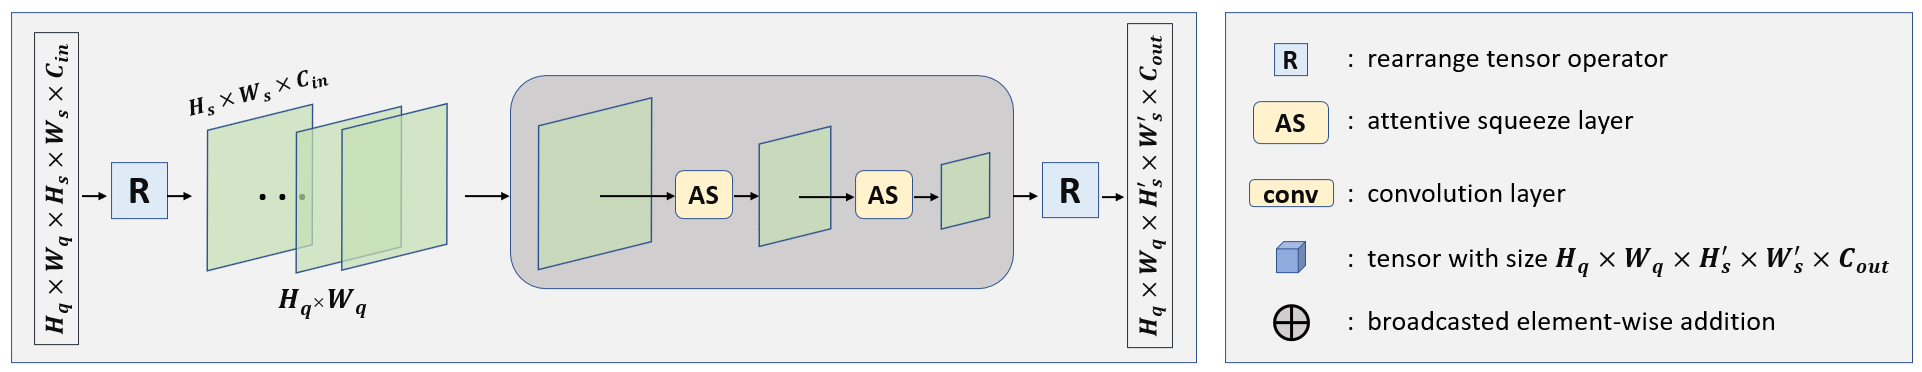
\includegraphics[width=\linewidth]{Fig/ASblock_and_legend.png}  
  \caption{The attentive squeeze block (AS block). Here, the legend placed at the right side is universal for all Figs. \ref{fig:asblock}, \ref{fig:cf}, and \ref{fig:bs}.}
  \label{fig:asblock}
\end{subfigure}
\begin{subfigure}{\textwidth}
  \centering
  % include second image
  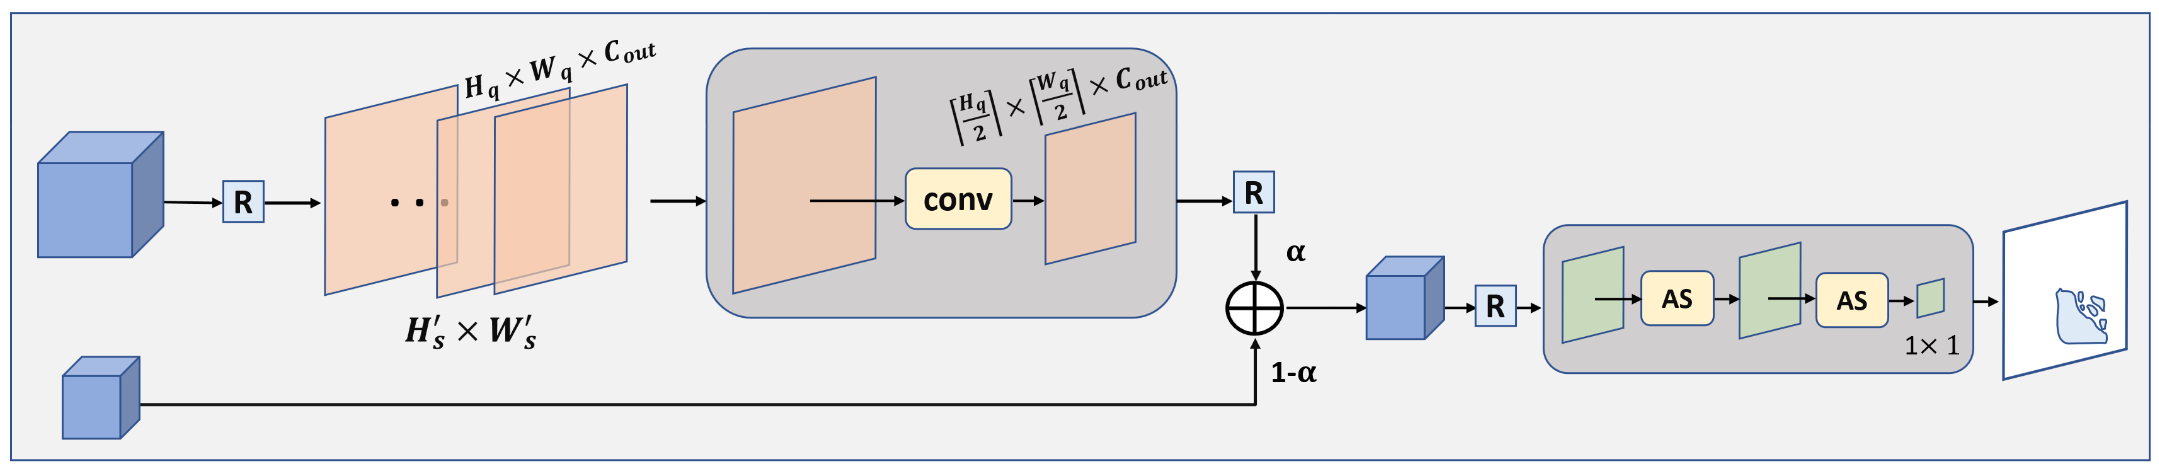
\includegraphics[width=\linewidth]{Fig/CFlayer_L.png}  
  \caption{Cross feature layer (CF layer).}
  \label{fig:cf}
\end{subfigure}
\begin{subfigure}{\textwidth}
  \centering
  % include second image
  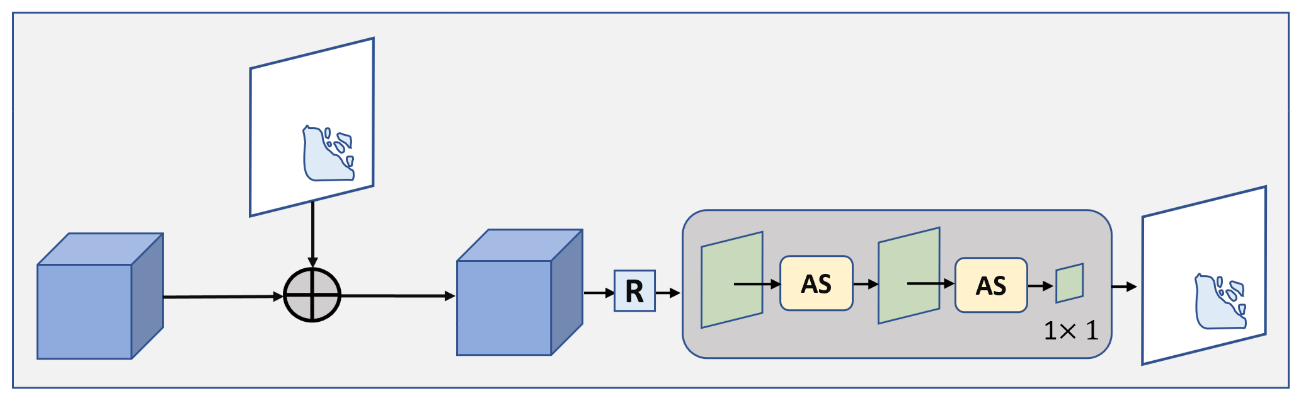
\includegraphics[width=0.6\linewidth]{Fig/BSlayer_L.png}  
  \caption{Broadcast and squeeze layer (BS layer).}
  \label{fig:bs}
\end{subfigure}
\caption{The architecture of the attentive squeeze block, cross feature layer, and broadcast and squeeze layer.}
\label{fig:fig}
\end{figure*}   

    
%We can consider it as a block matrix with size $H_{\mathrm{q}} \times W_{\mathrm{q}}$, and each element corresponding to a correlation tensor between each query position $x_q \in [H_{\mathrm{q}}] \times [W_{\mathrm{q}}]$ and every support position $\mathbf{C}\left(\mathbf{x}_{\mathrm{q}}\right) \in \mathbb{R}^{H_{\mathrm{s}} \times W_{\mathrm{s}} \times C_{\text {in }}}$}
\subsubsection{Cross Feature Layer}
\label{CFlayer}
In our study, via empirical experiments, we find that in many cases, the predicted road segmentation encroaches into the ground truth segmentation of the landslide. This observation is due to the fact that the landslide area is quite small compared to the road area and the whole image. Therefore, we propose cross feature layers (CF layers) between two adjacent correlations in a high-level correlation pyramid to enhance the model's ability to segment small objects.

In more detail, CF layers take as input two high-level correlation tensors $\mathbf{\ddot{\mathfrak{C}}}^{(b-1)}, \mathbf{\ddot{\mathfrak{C}}}^{(b)}$ $(b = 3,4)$ with size are $H_{q} \times W_{q} \times H^{'}_{s} \times W^{'}_{s} \times C_{out}$ and $\lceil \frac{H_{q}}{2} \rceil \times \lceil \frac{W_{q}}{2} \rceil \times H^{'}_{s} \times W^{'}_{s} \times C_{out}$,  respectively. First, we rearrange the bigger tensor $\mathbf{\ddot{\mathfrak{C}}}^{(b-1)}$ as a matrix block of size $H^{'}_{s} \times W^{'}_{s}$ with each elements size $H_{q} \times W_{q} \times C_{out}$. The elements then go through convolution layers for downsizing to the query dimension of the smaller tensor $\mathbf{\ddot{\mathfrak{C}}}^{(b)}$. Then, the result is rearranged and combined with the smaller tensor in the ratio $\alpha$, which shall be empirically determined via experiments. The mixed representation is rearranged and then fed to two sequential AS layers until it becomes a point feature of size $1 \times 1$. The detailed architecture of CF layers is illustrated in Fig. \ref{fig:cf}.

\subsubsection{Broadcast and Squeeze Layer}
\label{BSlayer}
For each high-level correlation $\mathbf{\ddot{\mathfrak{C}}}^{(b)}$ ($b=3,4$), after processing through CF layers, we have a feature map with the same size as the query dimension of the correlation $\mathbf{\ddot{\mathfrak{C}}}^{(b)}$. We then bi-linear upsampling that maps to the size of query dimension of $\mathbf{\ddot{\mathfrak{C}}}^{(b-1)}$. Next, the resulted map and the correlation $\mathbf{\ddot{\mathfrak{C}}}^{(b-1)}$ are input to the broadcast and squeeze layer (BS layer). The layer first uses broadcasted element-wise addition operator to combine the two inputs, then rearrange the resultant and finally feed the results to two sequential AS layers until the output becomes a point feature of size $1 \times 1$. Fig. \ref{fig:bs} illustrates the detailed architecture of BS layers.
%\subsubsection{Attention Module}

\subsection{Training Procedure}
\subsubsection{Prediction}
After obtaining the set of class-wise foreground maps, $\mathcal{Y}$, we perform the prediction/inference step to archive the multi-hot class occurrence, $\hat{\mathbf{y}}_{\mathbf{C}}$ and the segmentation mask, $\hat{\mathbf{Y}}_{\mathbf{S}}$.

\textbf{For classification.} With each class probability map $\mathbf{Y}^{(n)}$, if the maximum value of the matrix is greater than a pre-defined threshold $\delta$, then it means that the object with class $n$ is in the query image:
\begin{equation}
\hat{\mathbf{y}}_{\mathbf{C}}^{(n)}=\left\{\begin{array}{l}
1 \text { if } \max _{\mathbf{p} \in[H] \times[W]} \mathbf{Y}^{(n)}(\mathbf{p}) \geq \delta \\
0 \text { otherwise, }
\end{array}\right.
\end{equation}
where $\mathbf{p}$ represents the position in the matrix.


\textbf{For segmentation.} We compute the final segmentation mask $\hat{\mathbf{Y}}_{\mathbf{S}}$ by choosing the class that has the highest probability, for each pixel position:
\begin{equation}
\hat{\mathbf{Y}}_{\mathbf{S}}(\mathbf{p})=\underset{n \in[N+1]}{\arg \max } \mathbf{Y}^{(n)}, %\{\mathbf{Y}^{(1)}(\mathbf{p}), ..., \mathbf{Y}^{(N)}(\mathbf{p}), \mathbf{Y}^{(N+1)}(\mathbf{p})\}
\end{equation}
where $\mathbf{Y}^{(N+1)}$ is the background probability map derived from the class-wise foreground maps, expressed as follows:
\begin{equation}
\mathbf{Y}^{(N+1)}=\frac{1}{N} \sum_{n=1}^{N}\left(\mathbf{1}-\mathbf{Y}^{(n)}\right).
\label{eq6}
\end{equation}



\subsubsection{Loss Function }
FS-CS learner use segmentation loss in training, which is formulated as the average cross-entropy between the class distribution at each individual position and its ground-truth segmentation annotation:
\begin{equation}
\mathcal{L}=-\frac{1}{(N+1)} \frac{1}{H W} \sum_{n=1}^{N+1} \sum_{\mathbf{p} \in[H] \times[W]} \mathbf{Y}_{\mathrm{gt}}^{(n)}(\mathbf{p}) \log \mathbf{Y}^{(n)}(\mathbf{p}),
\end{equation}
where $\mathbf{Y}_{\mathrm{gt}}$ denotes the ground-truth segmentation mask.%\congtt{why the loss is termed $\mathcal{L}_{\mathrm{S}}$? Is this loss only computed based on the support set?}


\section{Experimental Results}
\label{sec:guidelines}
\subsection{Baselines and Performance Metrics}

We compare our proposed method with four state-of-the-art approaches:
\begin{itemize}
    
    \item \textbf{Path Aggregation Network (PANet) \cite{Kaixin2019}}: PANet reaches 1st place in the COCO 2017 Challenge Instance Segmentation task and 2nd place in the Object Detection task without large-batch training.
    
    \item \textbf{Prior Guided Feature Enrichment Network (PFENet) \cite{PFENet}} is one of state-of-the-art FSL methods.
    
    \item \textbf{Hypercorrelation Squeeze Networks (HSNet) \cite{HSNet}} is a novel framework for FS-CS that analyzes complex feature correlations in a fully-convolutional manner using light-weight 4D convolutions.
	
	\item \textbf{Attentive Squeeze Network (ASNet) \cite{Kang2022}}: This model achieves state-of-the-art performance on both FS-CS and FS-S tasks.
	
\end{itemize}

For multi-label classification evaluation metrics, we use the $0 / 1$ exact ratio: $\mathrm{ER}=\mathds{1}\left[\hat{\mathbf{y}}_{\mathbf{C}}=\right.$ $\mathbf{y}_\mathbf{gt}$ ], where $\mathbf{y}_{\mathrm{gt}}$ is the ground truth multi-hot class occurrence vector and $\hat{\mathbf{y}}_\mathbf{C}$ is predicted vector of the model.   For segmentation, we use mean IoU: $\mathrm{mIoU}=\frac{1}{N} \sum_{n} \operatorname{IoU}_{n}$, where $\mathrm{IoU}_{n}$ denotes an IoU \cite{iou} value of $n_{\text {th }}$ class.

\subsection{Experimental Setup}
We choose ResNet50 and ResNet101 trained on ImageNet as our backbone networks for comparison with other methods. The CF-ASNet is trained using the Adam optimizer\cite{kingma2014adam} with a learning rate of $10^{-4}$ for label segmentation. We train the model with two cases, 1-way 1-shot, and 2-way 1-shot. 



\subsection{Experimental Results}

In this section, we are interested in the following five research questions and we design experiments to investigate the answers to these questions.

% \datta{
\begin{itemize}
    \item[Q1.] How do different data augmentation methods affect performance?
    
    \item[Q2.] How much does CF-ASNet improve the performance on the LandslidePTIT dataset in comparison with other baselines?
    
    \item[Q3.] What is the performance of CF-ASNet and baselines with respect to the number of ways?
    
    \item[Q4.] How do the hyperparameters $\alpha$ and $\delta$ affect the performance of the CF-ASNet model?
    \item[Q5.] How close is the prediction of the CF-ASNet model to the ground truth?
    
    % \item \textit{Q3.} \datta{What are the differences or similarities between with recent FS-S methods on FS-S, and with recent FS-C methods on FS-C?}
\end{itemize}
% }

\subsubsection{Comparison of two data generation methods (Q1):}

\begin{table*}[t]
\caption{Results on few-shot learning of the proposed models}
\centering
\parbox[t]{\linewidth}{
\resizebox{\textwidth}{!}{
\begin{tabular}{|c|cccc|cccc|}
\hline
\textbf{}       & \multicolumn{4}{c|}{Dataset LB}                                                                          & \multicolumn{4}{c|}{Dataset LN}                                                                          \\ \hline
method & \multicolumn{2}{c|}{1-way 1-shot}                                 & \multicolumn{2}{c|}{2-way 1-shot}            & \multicolumn{2}{c|}{1-way 1-shot}                                 & \multicolumn{2}{c|}{2-way 1-shot}            \\ \hline
metric & \multicolumn{1}{c|}{cls. 0/1 ER} & \multicolumn{1}{c|}{seg. mIoU} & \multicolumn{1}{c|}{cls. 0/1 ER} & seg. mIoU & \multicolumn{1}{c|}{cls. 0/1 ER} & \multicolumn{1}{c|}{seg. mIoU} & \multicolumn{1}{c|}{cls. 0/1 ER} & seg. mIoU \\ \hline
PANet \cite{Kaixin2019}  & \multicolumn{1}{c|}{70. 6}       & \multicolumn{1}{c|}{31.0}      & \multicolumn{1}{c|}{62.2}        & 32.7      & \multicolumn{1}{c|}{63.36}       & \multicolumn{1}{c|}{23.6}      & \multicolumn{1}{c|}{53.4}        & 25.1      \\ \hline
PFENet \cite{PFENet} & \multicolumn{1}{c|}{75.9}        & \multicolumn{1}{c|}{35.1}      & \multicolumn{1}{c|}{61.7}        & 32.2      & \multicolumn{1}{c|}{62.8}        & \multicolumn{1}{c|}{27.3}      & \multicolumn{1}{c|}{46.5}        & 24.9      \\ \hline
HSNet \cite{HSNet}  & \multicolumn{1}{c|}{78.5}          & \multicolumn{1}{c|}{36.2}          & \multicolumn{1}{c|}{64.5} & \textbf{34.6} & \multicolumn{1}{c|}{64.0}          & \multicolumn{1}{c|}{28.8}          & \multicolumn{1}{c|}{\textbf{62.1}} & 28.0          \\ \hline
ASNet \cite{Kang2022} & \multicolumn{1}{c|}{80.4} & \multicolumn{1}{c|}{\textbf{38.5}} & \multicolumn{1}{c|}{64.2}          & 33.4          & \multicolumn{1}{c|}{66.7} & \multicolumn{1}{c|}{31.1} & \multicolumn{1}{c|}{61.7}          & \textbf{28.5} \\ \hline
CF-ASNet  & \multicolumn{1}{c|}{\textbf{81.4}} & \multicolumn{1}{c|}{\textbf{38.5}} & \multicolumn{1}{c|}{\textbf{65.3}}          & 34.1          & \multicolumn{1}{c|}{\textbf{68.8}} & \multicolumn{1}{c|}{\textbf{31.5}} & \multicolumn{1}{c|}{61.9}          & 27.7 \\ \hline
\end{tabular}
}
}
\label{tab:two-dataset}
\end{table*}


To validate the effectiveness of the proposed data generation method presented in Section \ref{sec:3}, we first train our model based on two datasets created by two variants of the data generation procedure as follows:
\begin{itemize}
    \item (1) \textit{LandslidePTIT dataset:} We insert landslide as described in Section \ref{sec:3}.
    \item (2) \textit{Dataset Landslide-Normal (LN):} We insert the landslide on the designated location of the image containing roads. 
\end{itemize}
Then, we evaluate the performance of all methods on another real-world data from \cite{landslide_2stage}, termed Landslide-Premise, which consists of 400 real-world landslide images captured by UAVs. That is, Landslide-Premise dataset acts as the test data. Table \ref{tab:two-dataset} shows the experimental results of all few-shot models, including CF-ASNet and competitive baselines trained on the two datasets that we created.

\begin{itemize}
    \item Performance of all models trained using \textit{LandslidePTIT dataset} are higher than that when training with \textit{LN} in both classification and data segmentation tasks. Therefore, the use of blending will affect the accuracy of the data classification model.
    \item We illustrate the qualitative result of two datasets in Fig. \ref{fig:LBvsLN}. As shown in Fig. \ref{fig:LB}, the landslide  overwritten on the original image using (1) is blended to make the data smoother and more realistic. As for (2), the included landslide  in Fig. \ref{fig:LN} looks coarser and does not look like a normal landslide.
\end{itemize}

Overall, we can see that the proposed data generation method achieves better results on actual data, showing the applicability of using this synthetic dataset as training data. 

\begin{figure}
    %\centering
    \begin{subfigure}[b]{0.47\linewidth}        %% or \columnwidth
        \centering
        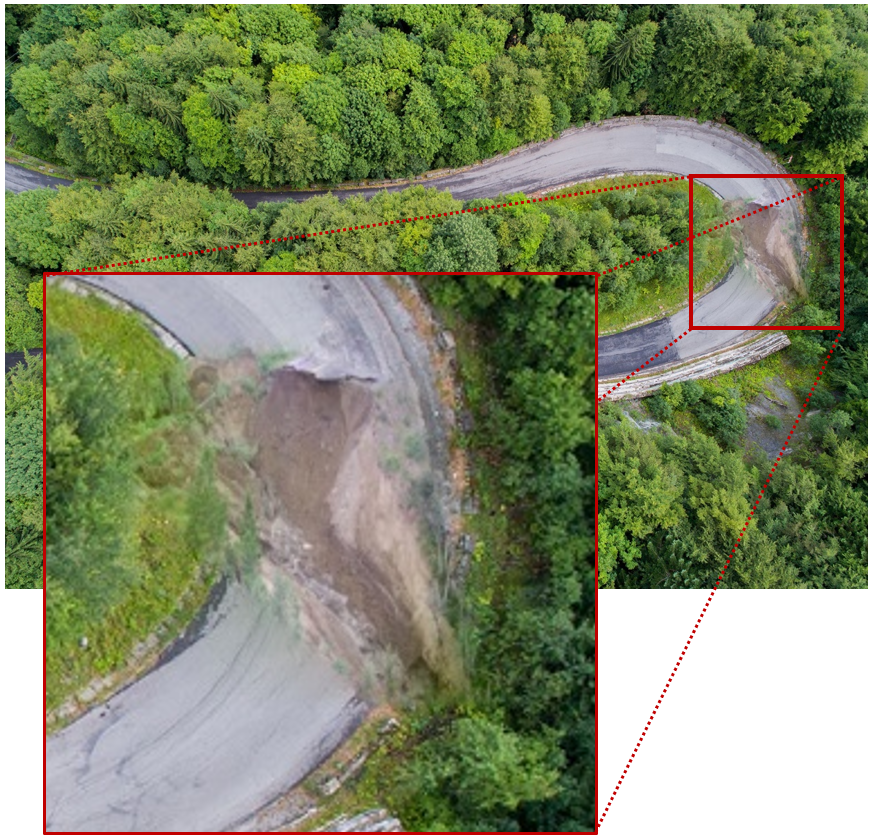
\includegraphics[width=\linewidth]{Fig/LB.png}
        \caption{An image from LandslidePTIT}
        \label{fig:LB}
    \end{subfigure}
    \hfill
    \begin{subfigure}[b]{0.47\linewidth}        %% or \columnwidth
        \centering
        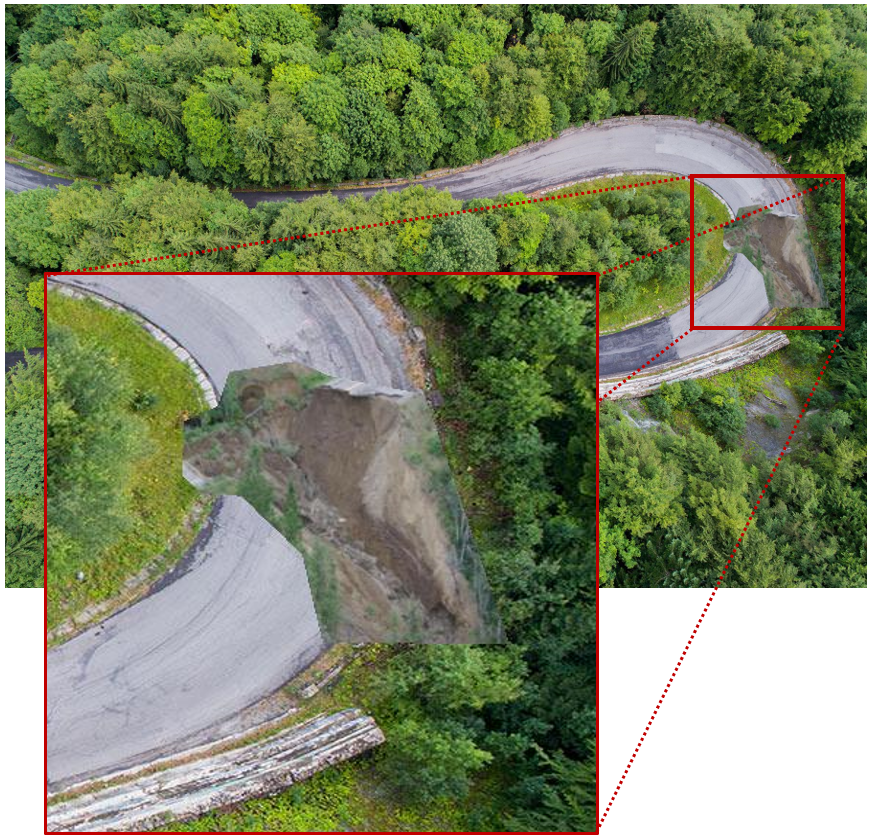
\includegraphics[width=\linewidth]{Fig/LN.png}
        \caption{An image from LN}
        \label{fig:LN}
    \end{subfigure}
    \caption{Visual comparison between the two generation methods.}
    \label{fig:LBvsLN}
\end{figure}

\subsubsection{Performance comparison of CF-ASNet and other baselines (Q2):}
From this part onwards, we use the LandslidePTIT dataset for both training and evaluation as this dataset is larger and more diverse than the Landslide-Premise dataset, making it more reasonable to evaluate competitive models. In this part, we divide LandslidePTIT into train and test sets. The train set consists of 1893 images that belong to 4 classes including Rockfall, Mudslide, Earth flow, and Road, in which the backgrounds of Roads are {\em Forest only} and {\em Forest mountain}. The test set contains 1070 images with two classes Depression and Road with {\em Rock mountain} background, respectively.

\begin{table}[h]
\caption{Performance comparison of CF-ASNet and others on our LandslidePTIT dataset}
\centering
\begin{tabular}{|ccccc|}
\hline
\multicolumn{5}{|c|}{Performance results}                                                                                                                        \\ \hline
\multicolumn{1}{|c|}{methods}  & \multicolumn{2}{c|}{1-way 1-shot}                                         & \multicolumn{2}{c|}{2-way 1-shot}                    \\ \hline
\multicolumn{1}{|c|}{metric}   & \multicolumn{1}{c|}{cls. 0/1 ER}    & \multicolumn{1}{c|}{seg. mIoU}      & \multicolumn{1}{c|}{cls. 0/1 ER}    & seg. mIoU      \\ \hline
\multicolumn{1}{|c|}{PANet}    & \multicolumn{1}{c|}{73.36}          & \multicolumn{1}{c|}{40.99}          & \multicolumn{1}{c|}{61.5}           & 38.42          \\ \hline
\multicolumn{1}{|c|}{PFENet}   & \multicolumn{1}{c|}{76.45}          & \multicolumn{1}{c|}{38.54}          & \multicolumn{1}{c|}{63.55}          & 36.85          \\ \hline
\multicolumn{1}{|c|}{HSNet}    & \multicolumn{1}{c|}{80.94}          & \multicolumn{1}{c|}{40.18}          & \multicolumn{1}{c|}{62.9}           & 41.26          \\ \hline
\multicolumn{1}{|c|}{ASNet}    & \multicolumn{1}{c|}{82.43}          & \multicolumn{1}{c|}{44.29}          & \multicolumn{1}{c|}{63.74}          & \textbf{42.42} \\ \hline
\multicolumn{1}{|l|}{CF-ASNET} & \multicolumn{1}{c|}{\textbf{83.21}} & \multicolumn{1}{c|}{\textbf{44.75}} & \multicolumn{1}{c|}{\textbf{64.11}} & 42.3           \\ \hline
\end{tabular}
\label{tab:model-eval}
\end{table}

\begin{figure*}
  \begin{subfigure}{\columnwidth}
  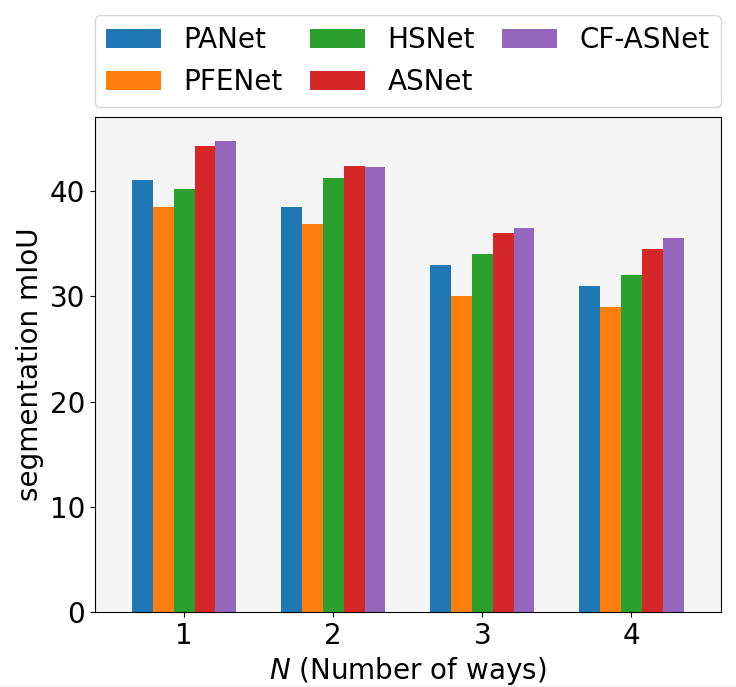
\includegraphics[width=0.95\textwidth]{Fig/4way_iou_2.png}
  \caption{Segmentation (mIoU)}
  \label{fig:compare-way-a}
  \end{subfigure}
  \hfill
  \begin{subfigure}{\columnwidth}
  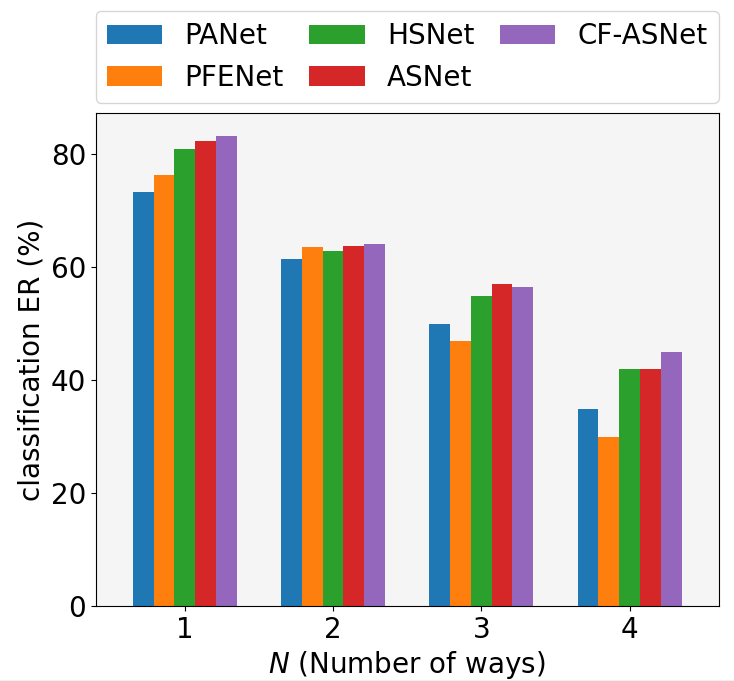
\includegraphics[width=0.95\textwidth]{Fig/4way_er_2.png}
  \caption{Classification (exact ratio)}
  \label{fig:compare-way-b}
  \end{subfigure}
  \caption{$N$-way 1-shot FS-CS performance comparison of five
methods by varying $N$ from 1 to 4 on LandslidePTIT}
  \label{fig:compare-way}
\end{figure*}

\begin{figure*}
  \centering
  \begin{subfigure}{\columnwidth}
  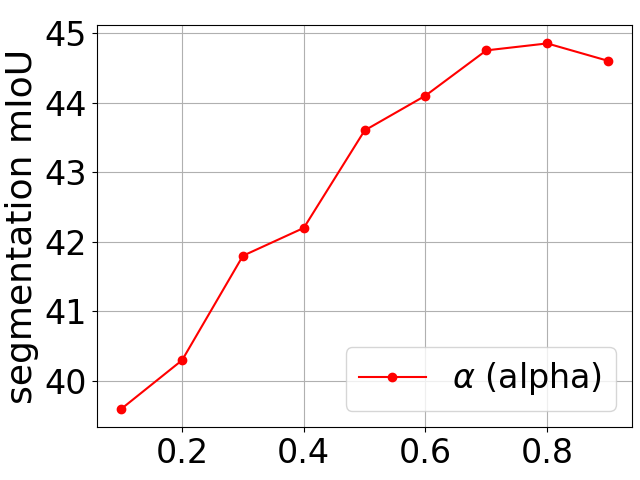
\includegraphics[width=0.49\textwidth]{Fig/alpha_iou_3.png}
  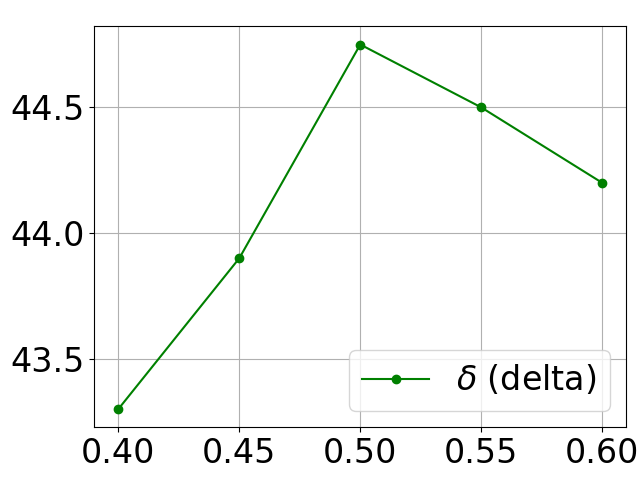
\includegraphics[width=0.49\textwidth]{Fig/delta_iou.png}
  \caption{Segmentation (mIoU)}
  \label{fig:alpha-a}
  \end{subfigure}
  \hfill
  \begin{subfigure}{\columnwidth}
  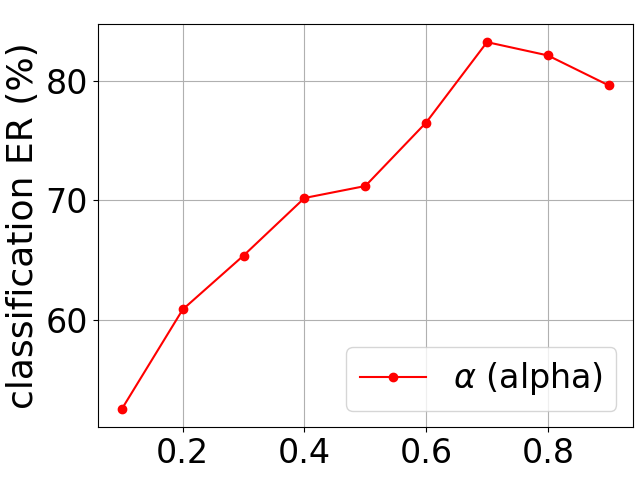
\includegraphics[width=0.49\textwidth]{Fig/alpha_er_3.png}
  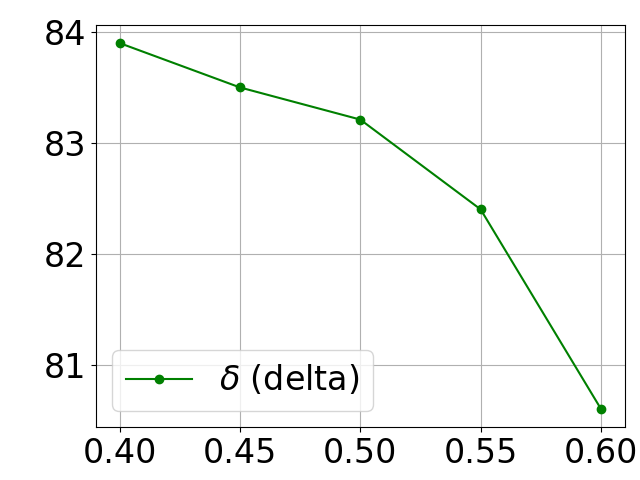
\includegraphics[width=0.49\textwidth]{Fig/delta_er.png}
  \caption{Classification (exact ratio)}
  \label{fig:alpha-b}
  \end{subfigure}
  \caption{Performance of 1-way 1-shot CF-ASNet on LandslidePTIT when varying $\alpha$ and $\delta$}
  \label{fig:alpha}
\end{figure*}



Table \ref{tab:model-eval} presents the performance for both classification and segmentation tasks of all competitive schemes, including PANet, PFENet, HSNet, ASNet, and our proposed method CF-ASNet. We discuss interesting points as follows.
\begin{itemize}
    \item We find that our CF-ASNet model achieves the best performance in terms of both 0/1 ER and mIoU among all the few-shot learning models in the 1-way 1-shot setting. Notably, the performance of CF-ASNet achieves 1\% higher ER and 0.5\% higher mIoU than the results obtained by ASNet, accounting for the contribution of the new cross-feature layer.
    \item The performance of CF-ASNet is much higher than those of PANet and HSNet, with the gain from 10 to 15\% with the classification metric 0/1 ER, and from 3 to 7\% with the segmentation metric mIoU. This is due to the well-designed architecture including the combination of ASNet and hypercorrelation computation.
\end{itemize}




% \subsubsection{Comparison with recent FS-S methods on FS-S, and with recent FS-C methods on FS-C}

% \datta{}


\subsubsection{Comparison between all competitive schemes with respect to the number of ways (Q3):}

In Fig. \ref{fig:compare-way}, we perform an experiment where the number of ways is adjustable. In the case when the number of ways is 1, we randomly choose a type of landslide to put in the test set. When the number of ways $N > 1$, i.e., $N\in\{2,3,4\}$, we randomly divide the classes of the training set to include $N-1$ landslide labels, which means the test set includes $4-(N-1)$ other labels of landslide. 

As shown in Fig. \ref{fig:compare-way-a}, in the case of 1-way 1-shot,  our CF-ASNet method works best with an accuracy of 81\%. Besides, we also notice a decrease in both ER and mIoU as we increase the number of ways from 1 to 4. Overall, the performance of CF-ASNet is always the highest, except for the case where $N$ is set to 3, where the performance of ASNet is slightly superior. 

In Fig. \ref{fig:compare-way-b}, we illustrate the superiority of CF-ASNet for the segmentation task when varying the number of ways. 

\subsubsection{Hyperparameter Sensitivity Analysis (Q4):}

 In Fig. \ref{fig:alpha}, we present the  sensitivity analysis of the parameters $\alpha$ of the Cross Feature Layer and threshold  $\delta$ of the prediction. When analyzing $\alpha$, we set the default value of $\delta$ as 0.5 in all experiments. 
 
 When we increase $\alpha$ from 0.1 to 0.7,  the performance of both segmentation and classification tasks exhibits an upward trend. As shown in Fig. \ref{fig:alpha-a}, with $\alpha$ = 0.8, the segmentation mIoU value reaches the highest value (approximately 45). In Fig. \ref{fig:alpha-b}, when we set $\alpha$ to 0.7, the accuracy of the classification model peaked at approximately 82\%. In general, we empirically find that when $\alpha$ ranges from 0.7 to 0.8, the model performs well. We note that we can validate the choice of parameter $\alpha$ using various validation methods such as k-fold validation.

Next, we adjust the threshold coefficient $\delta$ while the parameter $\alpha$ is set to 0.7. When $\delta< 0.5$, the ER is high and the mIoU is at a lower value. When  $\delta > 0.5$, the mIoU experiences a decrease while ER also drops. In our experiment, we set the threshold $\delta=0.5$.

\subsubsection{Qualitative Study (Q5):}

    \begin{figure*}[t]
        \centering
        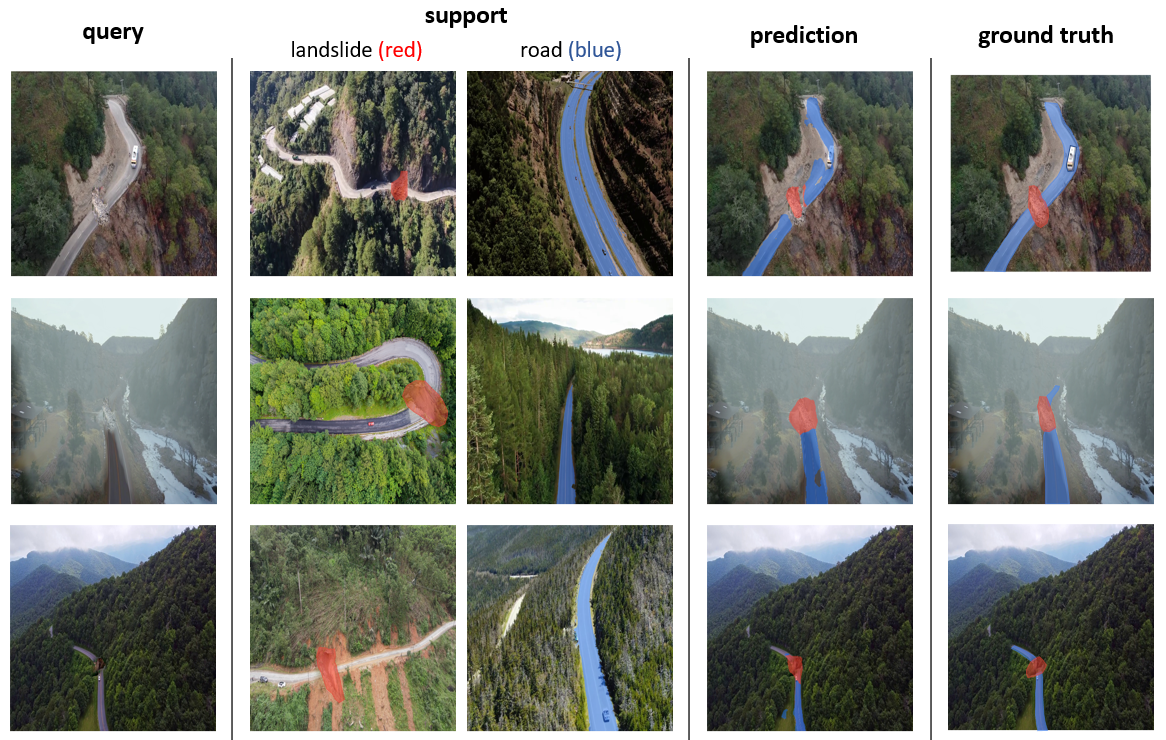
\includegraphics[width=\textwidth]{Fig/quali_study.png}
        \caption{The prediction of CF-ASNet model}
        \label{fig:demo}
    \end{figure*}

We perform the qualitative study by showing the results obtained from the CF-ASNet model, in the form of landslide images captured by drones in Fig. \ref{fig:demo}. The CF-ASNet model takes two sets, including query and support sets, as the input. On the left side of Fig. \ref{fig:demo}, we illustrate the query sets that are images extracted from LandslidePTIT. In the middle of the figure, we show examples of the support set used in the training process, where red and blue marks represent the pixels containing the landslide and the road, respectively. The prediction result of CF-ASNet model is displayed on the right side of the figure, side-by-side with the ground-truth images. From the example, one can see that the CF-ASNet model provides well-segmented roads and landslides. 

\section{Conclusion}

In this study, we introduced a swift detection system that can locate the occurrence of landslides on roads. Due to the difficulties in data collection of real-world landslide images, the system was trained upon a synthetic dataset, created from our new design procedure. We also proposed a new few-shot segmentation method, termed CF-ASNet, to enhance the capacity of the system in detecting landslides in real-world situations. Experimental results showed promising applicability of the generated dataset as well as the proposed CF-ASNet model in classifying and segmenting damages caused by landslides on roads.

Future avenues include the enrichment of the synthetic dataset using additional  real-world conditions and terrains. We also plan to conduct an empirical study when deploying this system in the mountainous areas of Vietnam.

% \bibitem{sat-lo-2022} Serious landslide on the route Da Lat - Mui Ne. [Online].
% Available: https://vnexpress.net/sat-lo-nghiem-trong-tren-tuyen-da-lat-mui-ne-4465736.html

% \bibitem{Bourenane2021} H. Bourenane and Y. Bouhadad, “Impact of Land use Changes on Landslides Occurrence in Urban Area: The Case of the Constantine City (NE Algeria),” Geotech. Geol. Eng., vol. 39, no. 6, 2021, doi: 10.1007/s10706-021-01768-1.

% \bibitem{Picarelli2021} L. Picarelli, S. Lacasse, and K. K. S. Ho, The Impact of Climate Change on Landslide Hazard and Risk. Springer International Publishing, 2021.

% \bibitem{Hung2015} Manh Hung Nguyen, Tuong Vinh Ho, Trong Khanh Nguyen and Minh Duc Do, “Modeling and simulation of the effects of landslide on circulation of transports on the mountain roads” International Journal of Advanced Computer Science and Applications(ijacsa), 6(8), 2015. http://dx.doi.org/10.14569/IJACSA.2015.060835

% \bibitem{Ma2021} Z. Ma, G. Mei, and F. Piccialli, “Machine learning for landslides prevention: a survey,” Neural Comput. Appl., vol. 33, no. 17, pp. 10881–10907, 2021, doi: 10.1007/s00521-020-05529-8. 

% \bibitem{Tehrani2022} F. S. Tehrani, M. Calvello, Z. Liu, and L. Zhang, Machine learning and landslide studies : recent advances and applications, no. 0123456789. Springer Netherlands, 2022.

% \bibitem{Li2022} X. Li, J. Cheng, and D. Yu, “Research on Landslide Risk Assessment Based on Convolutional Neural Network,” pp. 8–12, 2022, doi: 10.1109/LGRS.2022.3185052.

% \bibitem{Kang2022} D. Kang and M. Cho, “Integrative Few-Shot Learning for Classification and Segmentation,” Cvpr, 2022, [Online]. Available: http://cvlab.postech.ac.kr/research/iFSL.

% \bibitem{Prakash2021}N. Prakash, A. Manconi, and S. Loew, “A new strategy to map landslides with a generalized convolutional neural network,” Sci. Rep., vol. 11, no. 1, pp. 1–15, 2021, doi: 10.1038/s41598-021-89015-8.

% \bibitem{Ghorbanzadeh2021}O. Ghorbanzadeh, A. Crivellari, P. Ghamisi, H. Shahabi, and T. Blaschke, “A comprehensive transferability evaluation of U-Net and ResU-Net for landslide detection from Sentinel-2 data (case study areas from Taiwan, China, and Japan),” Sci. Rep., vol. 11, no. 1, pp. 1–20, 2021, doi: 10.1038/s41598-021-94190-9.








% \bibitem{HongYu2017} Hong Yu, Yi Ma, Longfei Wang, Yongsai Zhai and Xiaoqian Wang, "A landslide intelligent detection method based on CNN and RSG-R", Published 1 August 2017 Computer Science 2017 IEEE International Conference on Mechatronics and Automation (ICMA)
% \bibitem{Haojie2021} Haojie Wanga, Limin Zhanga, Kesheng Yina, Hongyu Luoa, Jinhui Lib, "Landslide identification using machine learning". Geoscience Frontiers Volume 12, Issue 1, January 2021, Pages 351-364 
% \bibitem{Milos2009}Miloš Marjanoviü, Branislav Bajat, Miloš Kovaþeviü, "Landslide susceptibility assessment with machine learning algorithms". 2009 International Conference on Intelligent Networking and Collaborative Systems

% \bibitem{ChanW2014} Chen W, Li X, Wang Y, Chen G, Liu S (2014) Forested landslide detection using LiDAR data and the random forest algorithm: a case study of the Three Gorges. China Remote Sensing of Environment 152:291–301
% \bibitem{Chandra2012}Chandra Prakash Poudyal, Landslide susceptibility analysis using decision tree method, Phidim, Eastern Nepal. Bulletin of the Department of Geology, Tribhuvan University, Kathmandu, Nepal, Vol. 15, 2012, pp. 69–76
% \bibitem{Ilia2016}Paraskevas Tsangaratos, Loanna Ilia, Comparison of a logistic regression and Naïve Bayes classifier in landslide susceptibility assessments: The influence of models complexity and training dataset size. CATENA Volume 145, October 2016, Pages 164-179
% \bibitem{Lian2014} Cheng Lian, Zhigang Zeng, Wei Yao \& Huiming Tang, Extreme learning machine for the displacement prediction of landslide under rainfall and reservoir level. Stochastic Environmental Research and Risk Assessment volume 28, pages1957–1972 (2014)
% \bibitem{Badal2020} Badal Pokharel, Omar F. Althuwaynee, Ali Aydda, Sang-Wan Kim, Samsung Lim, Hyuck-Jin Park Spatial clustering and modelling for landslide susceptibility mapping in the north of the Kathmandu Valley, Nepal
% \bibitem{TrongAn2020}Trong-An Bui, Pei-Jun Lee, Kai-Yew Lum, Clarissa Loh, Kyo Tan, "Deep Learning for Landslide Recognition in Satellite Architecture".  IEEE Access(Volume: 8) 05 August 2020
% \bibitem{Anzi2016} Anzi Ding, Qingyong Zhang, Xinmin Zhou, and Bicheng Dai, "Automatic Recognition of Landslide Based on CNN and Texture Change Detection", 2016 31st Youth Academic Annual Conference of Chinese Association of Automation (YAC)
% \bibitem{Unet2015} Ronneberger O, Fischer P, Brox T (2015) U-Net: convolutional networks for biomedical image segmentation. International Conference on Medical image computing and computer-assisted intervention. Springer, pp 234–241

% \bibitem{HuajinLi2022} Huajin Li, Yusen He, Qiang Xu, Jiahao Deng, Weile Li and Yong Wei, "Detection and segmentation of loess landslides via satellite images: a two-phase framework", Springer-Verlag GmbH Germany, part of Springer Nature 2021 

% \bibitem{Sansar2022}Sansar Raj Meena, Lucas Pedrosa Soares, Carlos H. Grohmann, Cees van Westen, Kushanav Bhuyan, Ramesh P. Singh, Mario Floris \& Filippo Catani "Landslide detection in the Himalayas using machine learning algorithms and U-Net"

% \bibitem{Zhunli2020}Zhun Li, Yonggang Guo, "Semantic segmentation of landslide images in Nyingchi region based on PSPNet network". 2020 7th International Conference on Information Science and Control Engineering (ICISCE)
% \bibitem{Lucas2022}Lucas Pedrosa Soares ,Helen Cristina Dias ,Guilherme Pereira Bento Garcia  and Carlos Henrique Grohmann   "Landslide Segmentation with Deep Learning: Evaluating Model Generalization in Rainfall-Induced Landslides in Brazil" 6 May 2022 MDPI

% \bibitem{Kelsey2019}Kelsey Allen, Evan Shelhamer, Hanul Shin, and JoshuaTenenbaum. Infinite mixture prototypes for few-shot learn-ing. In Proc. International Conference on Machine Learn-ing (ICML), 2019

% \bibitem{Kaixin2019}Kaixin Wang, Jun Hao Liew, Yingtian Zou, Daquan Zhou Jiashi Feng, PANet: Few-Shot Image Semantic Segmentation with Prototype Alignment ICCV 2019
% \bibitem{Joaquin2018}Joaquin Vanschoren "Meta-Learning: A Survey" 8 October 2018 Computer Science, Biology ArXiv
% \bibitem{Mark2017}Mark Woodward, Chelsea Finn, "Active One-shot Learning". arXiv preprint arXiv:1702.06559, 2017
% \bibitem{Brenden2011}Brenden M. Lake, Ruslan Salakhutdinov, Jason Gross, and Joshua B. Tenenbaum "One shot learning of simple visual concepts" Proceedings of the Annual Meeting of the Cognitive Science Society, 33(33) 2011
% \bibitem{Fei2006}Li Fei-Fei, R. Fergus, P. Perona "One-Shot Learning of Object Categories".  IEEE Transactions on Pattern Analysis and Machine Intelligence ( Volume: 28, Issue: 4, April 2006)

% \bibitem{Lampert2013}C. Lampert, H. Nickisch, and S. Harmeling, “Attribute-based classification for zero-shot visual object categorization,” in TPAMI, 2013.

% \bibitem{Larochelle2008}H. Larochelle, D. Erhan, and Y. Bengio, “Zero-data learning of new
% tasks,” in AAAI, 2008.

% \bibitem{Rohrbach2011} M. Rohrbach, M. Stark, and B.Schiele, “Evaluating knowledge transfer
% and zero-shot learning in a large-scale setting,” in CVPR, 2011

% \bibitem{Ding2017}Z. Ding, M. Shao, and Y. Fu, “Low-rank embedded ensemble semantic
% dictionary for zero-shot learning,” in CVPR, 2017
% \bibitem{Dhillon2020}Guneet S. Dhillon, Pratik Chaudhari, Avinash Ravichandran, Stefano Soatto "A Baseline for Few-Shot Image Classification". ICLR 2020
% \bibitem{Chen2021}Da Chen, Yuefeng Chen, Yuhong Li, Feng Mao, Yuan He, Hui Xue "Self-Supervised Learning for Few-Shot Image Classification". ICASSP 2021 - 2021 IEEE International Conference on Acoustics, Speech and Signal Processing (ICASSP)
% \bibitem{Liu2019}Bing Liu; Xuchu Yu; Anzhu Yu; Pengqiang Zhang; Gang Wan; Ruirui Wang "Deep Few-Shot Learning for Hyperspectral Image Classification" IEEE Transactions on Geoscience and Remote Sensing ( Volume: 57, Issue: 4, April 2019)
% \bibitem{Majee2021}Anay Majee, Kshitij Agrawal, Anbumani Subramanian "Few-Shot Learning for Road Object Detection". Proceedings of Machine Learning Research 140:115–126, 2021 AAAI Workshop on Meta-Learning and MetaDL Challenge
% \bibitem{Das2019}Debasmit Das, C. S. George Lee "A Two-Stage Approach to Few-Shot Learning for Image Recognition"  IEEE Transactions on Image Processing ( Volume: 29)
% \bibitem{Boudiaf2021} Malik Boudiaf; Hoel Kervadec; Ziko Imtiaz Masud; Pablo Piantanida; Ismail Ben Ayed; Jose Dolz "Few-Shot Segmentation Without Meta-Learning: A Good Transductive Inference Is All You Need?" 2021 IEEE/CVF Conference on Computer Vision and Pattern Recognition (CVPR)
% \bibitem{Wang2019} Kaixin Wang, Jun Hao Liew, Yingtian Zou, Daquan Zhou, Jiashi Feng, "PANet: Few-Shot Image Semantic Segmentation with Prototype Alignment" ICCV 2019 

% \bibitem{Dong2018}Nanqing Dong, Eric P. Xing "Few-Shot Semantic Segmentation with Prototype Learning" BMVC2018

% \bibitem{liu2019roadnet}Liu, Yahui and Yao, Jian and Lu, Xiaohu and Xia, Menghan and Wang, Xingbo and Liu, Yuan "RoadNet: Learning to Comprehensively Analyze Road Networks in Complex Urban Scenes from High-Resolution Remotely Sensed Images" IEEE Transactions on Geoscience and Remote Sensing

% \bibitem{matias2016Poisson-Image-Editing}J. Matias Di Martino, Gabriele Facciolo, Enric Meinhardt-Llopis "Poisson Image Editing" IPOL 2016




% \bibliographystyle{ieeetr}
% \bibliography{refers}

\bibliographystyle{IEEEtran}
\bibliography{refers}


% \end{thebibliography}
% \bibliography{refer}
\begin{IEEEbiography}[{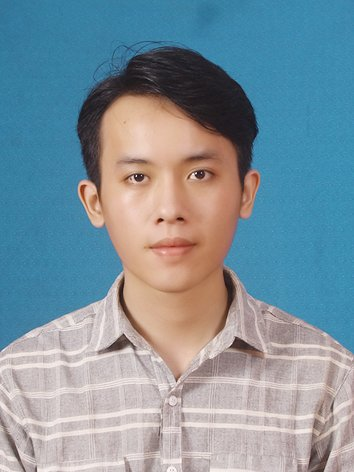
\includegraphics[width=1in,height=1.25in,clip,keepaspectratio]{Fig/datta.jpg}}]{Dat Tran-Anh} was born in Hanoi, Vietnam, in 1997. He received the B.E. degree in security information and M.S degree in computer science from Posts and Telecommunications Institute of Technology, Hanoi, in 2020 and 2022, respectively. He is currently an AI Engineer with MobiFone Infomation Technology Center. His research interests include image processing, signal preprocessing, and machine learning/deep learning.
\end{IEEEbiography}

\begin{IEEEbiography}[{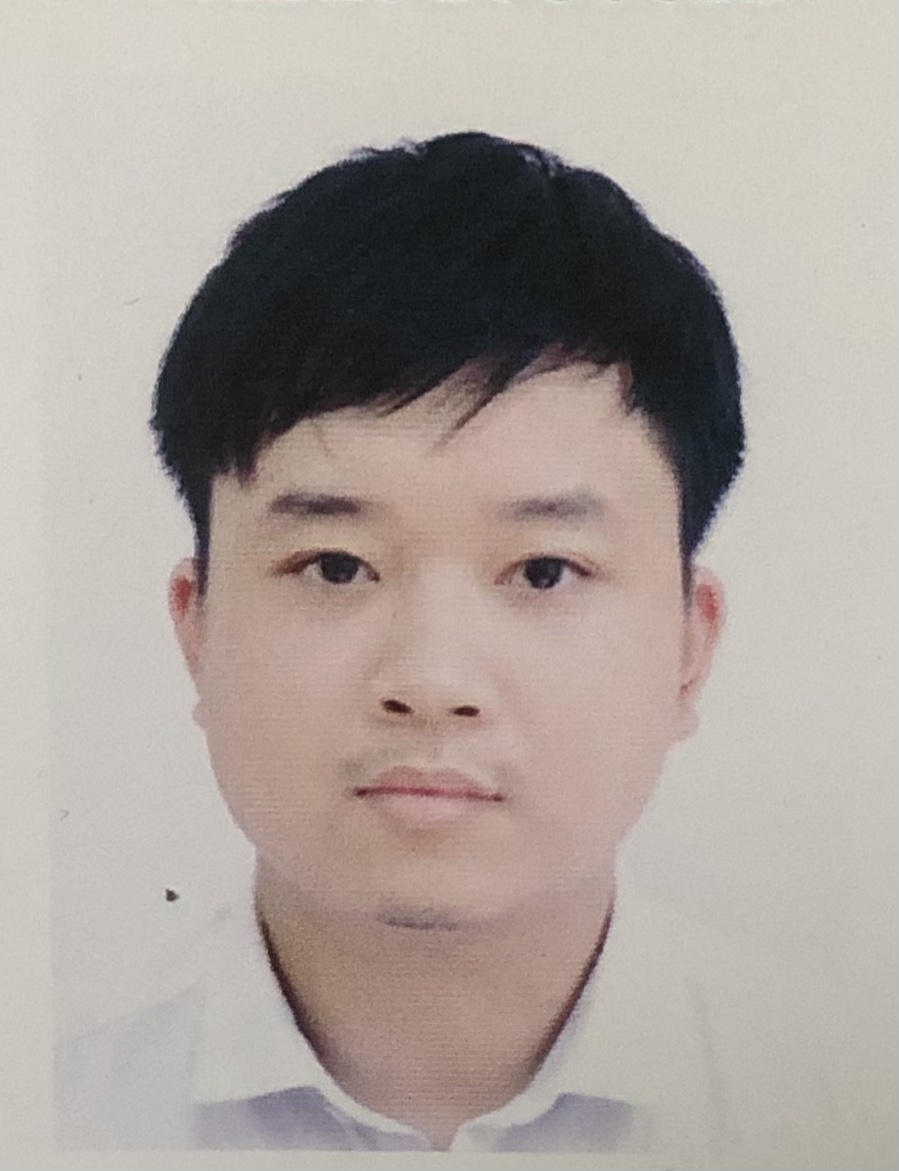
\includegraphics[width=1in,height=1.25in,clip,keepaspectratio]{Fig/baobq_c.jpg}}]{BAO BUI-QUOC} was born in Thai Binh, Viet Nam in 
1998. He received the B.E. degree in applied mathematics and informatics from 
Hanoi University of Science and Technology, Ha Noi, in 2021. He is currently an AI Engineer at MobiFone Infomation Technology Center. His research interests include image processing, computer vision, and machine learning/reinforcement learning.
\end{IEEEbiography}

\begin{IEEEbiography}[{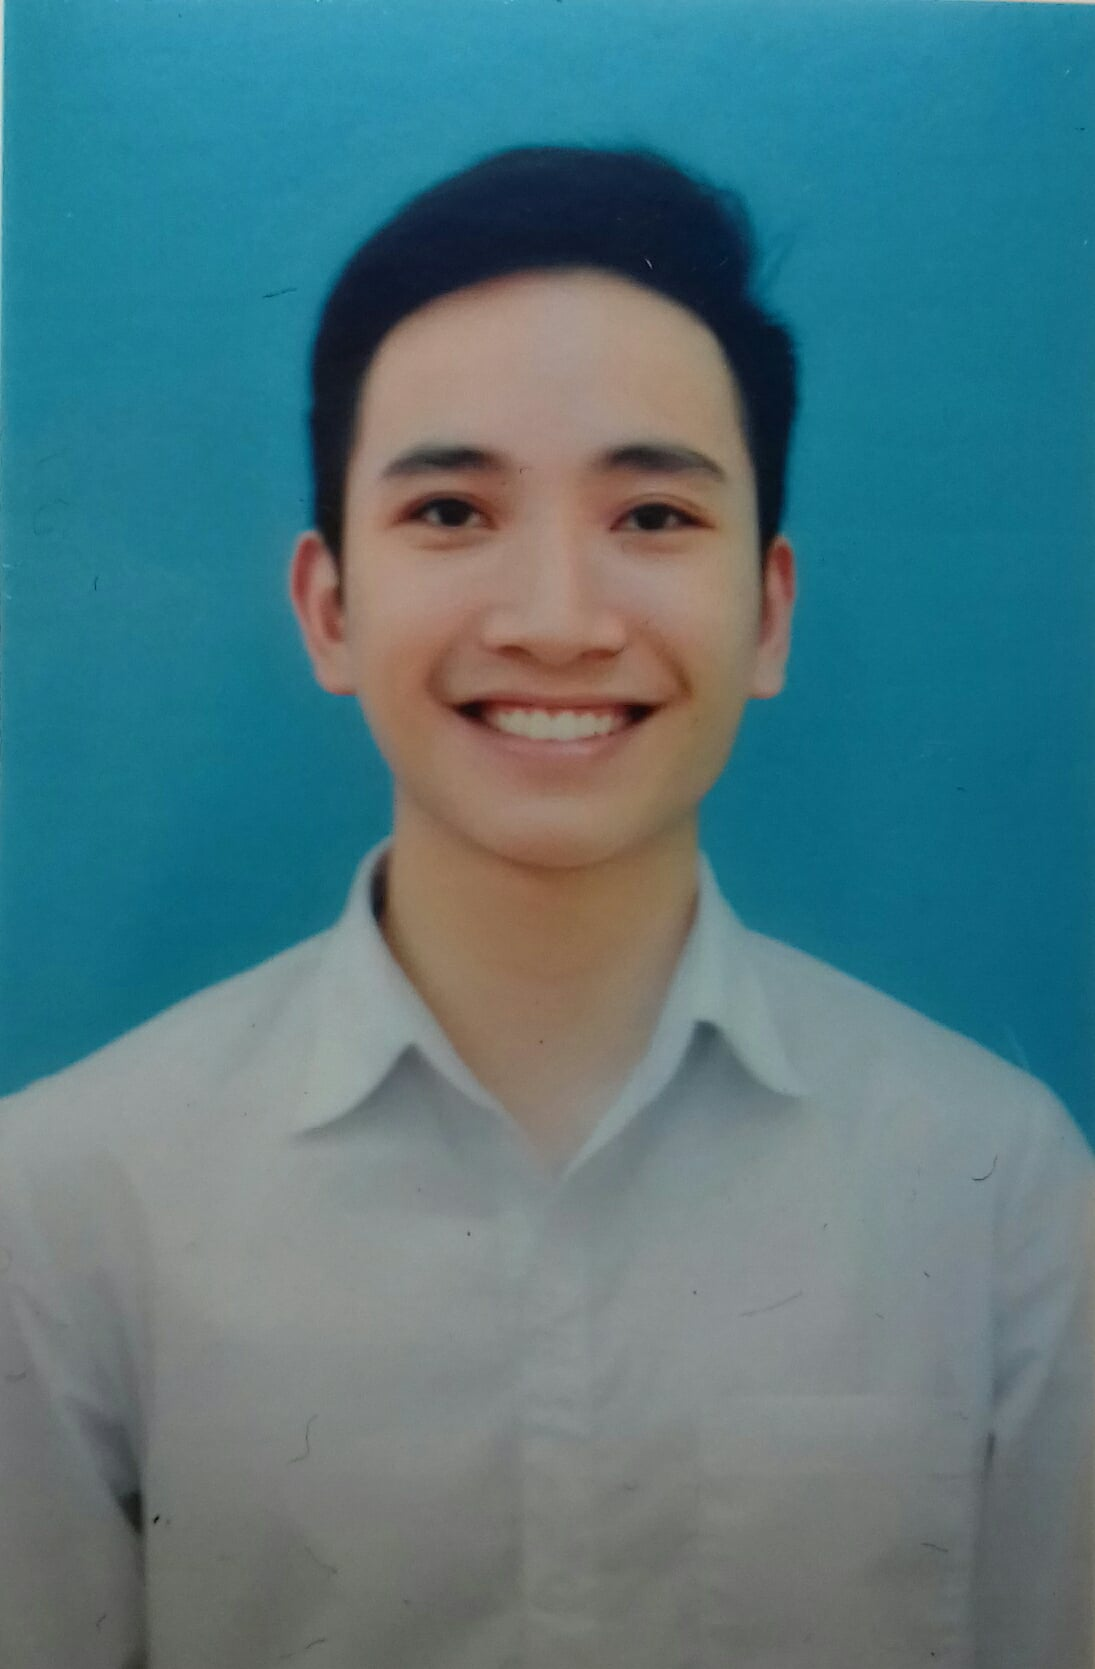
\includegraphics[width=1in,height=1.25in,clip,keepaspectratio]{anhthe.png}}]{ANH VU-DUC} was born in Hanoi, Vietnam, in 2000. He is a fourth-year student at Posts and Telecommunications Institute of Technology, Hanoi. His major is Computer Science and his research interests include image processing, computer vision, natural language processing, and machine learning/deep learning
\end{IEEEbiography}

\begin{IEEEbiography}[{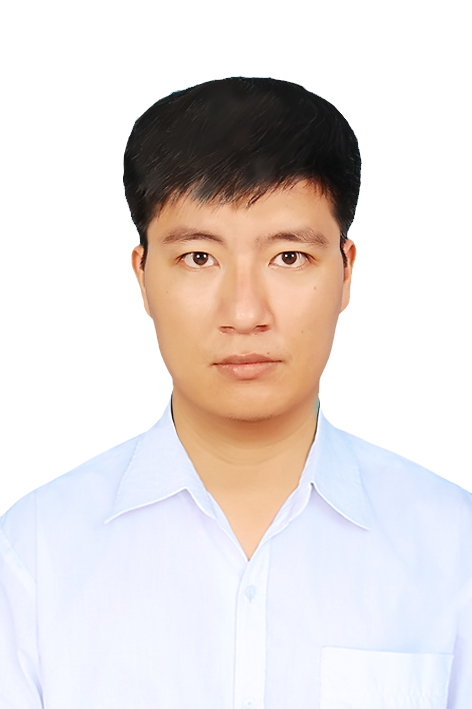
\includegraphics[width=1in,height=1.25in,clip,keepaspectratio]{Fig/TrungAnh.jpg}}]{TRUNG-ANH DO} received the B.S. and the M.S. degrees in telecommunications and electronics
engineering from the Hanoi University of Technology, Hanoi, Vietnam, in 2009 and 2011, respectively, and the Ph.D. degree
in telecommunications engineering from the Posts and Telecommunications Institute of Technology, Hanoi. From 2011 to 2014, he was a Researcher with the Research Institute of Posts and Telecommunications, Hanoi, Vietnam. From 2014 to 2016, he was
with the Communications \& Networking Laboratory, Dankook University, Yongin, South Korea. Since December 2016, he has been with The Department of Science \& Technology Management and International Cooperation, Posts and Telecommunications Institute of Technology, Hanoi, Vietnam.  His research interests include wireless communications, mobile computing, data mining, and machine learning
\end{IEEEbiography}

\begin{IEEEbiography}[{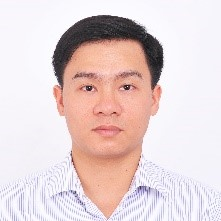
\includegraphics[width=1in,height=1.25in,clip,keepaspectratio]{Fig/Hung.jpg}}]{VIET-HUNG NGUYEN} received his MSc degree in 2009 from Grenoble Institute of Technology and his PhD in Signal Processing and Telecommunications from University of Rennes 1, France. He is currently a Lecturer at Posts and Telecommunications Institute of Technology, Vietnam. His research activities are focus on antennas and microwave circuit design for next-generation wireless communication systems. 
\end{IEEEbiography}

\begin{IEEEbiography}[{
\includegraphics[width=1in,height=1.25in,clip,keepaspectratio]{Fig/hoai.png}}]{Hoai Nam Vu} was born in Ha Noi, Viet Nam in 
1990. He received the B.E. degree in Electronic and Telecommunication Engineering from 
the Ha Noi University of Science and Technology, Ha Noi, Viet Nam in 2013 and the M.S. degree in 
Electronic and Computer engineering from Chonnam National University, Gwangju, South Korea, in 2015. He is currently pursuing the Ph.D. degree in Computer Science at Posts and Telecommunications Institute of Technology, Ha Noi.
Since 2016, he has been a lecturer with Computer Science Department, Posts and Telecommunications Institute of Technology, Viet Nam. His research interests include sensor signal processing, drone-based image processing, machine learning, and deep learning.
\end{IEEEbiography}


\begin{IEEEbiography}[{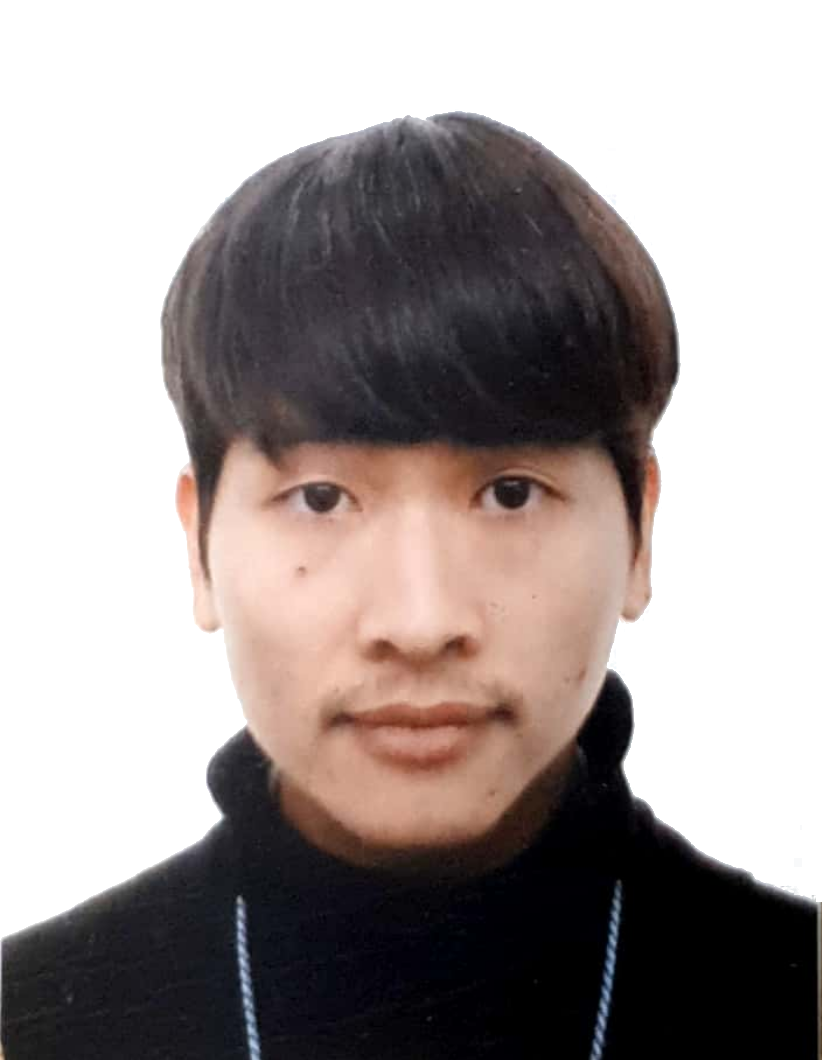
\includegraphics[width=1in,height=1.25in,clip,keepaspectratio]{Fig/Cong.png}}]{Cong Tran}  received his doctoral degree in computer science from Dankook University, Yongin,
Republic of Korea, in 2021. He previously received his M.Sc. in computer science in 2014 and his B.Sc. in network and communication in 2009 from Vietnam National University, Hanoi, Vietnam. Since September 2021, he has been with the Faculty of Information Technology, Posts \& Telecommunication Institute of Technology, Hanoi, Vietnam, as a lecturer. His research interests include social network analysis, data mining, and machine learning.
\end{IEEEbiography}
\EOD

\end{document}
sat-lo-2022